% Questo file definisce lo stile che verrà applicato
% ad ogni pagina di contenuto
\documentclass[a4paper,11pt]{article}

\usepackage{ifthen}
\usepackage[
 a4paper,
 top=2.5cm,
 bottom=2.5cm,
 left=1.5cm,
 right=1.5cm,
 head=30pt
]{geometry}
\usepackage[italian]{babel}
\usepackage[utf8x]{inputenc}
\usepackage[T1]{fontenc}
\usepackage{fancyhdr}
\usepackage[colorlinks=true, urlcolor=black, citecolor=black, linkcolor=black]{hyperref}
\usepackage{tabularx}
\usepackage{multirow}
\usepackage{booktabs}
\usepackage{color}
\usepackage[dvipsnames]{xcolor}
\usepackage{graphicx}
\usepackage{eurosym}
\usepackage{amsmath}
\usepackage{relsize}
\usepackage{placeins}
\usepackage{ltablex}
\usepackage{float}

\usepackage[multidot]{grffile}
\usepackage{xcolor,colortbl}
\definecolor{lightblue}{HTML}{56B4E6}
\definecolor{blue}{HTML}{2953A1}
\definecolor{darkblue}{HTML}{1E396E}
\usepackage{longtable}

\usepackage[toc,page]{appendix}
\renewcommand\appendixtocname{Appendice}
\renewcommand{\appendixpagename}{Appendice}

\newcommand\pagenumberingnoreset[1]{\gdef\thepage{\csname @#1\endcsname\c@page}}

% Cambia il font 
\renewcommand*\rmdefault{qhv}

% ***STILE PAGINA***
\pagestyle{fancy}
\fancyhf{}
\setlength{\headheight}{1cm} 
% No indentazione paragrafo
\setlength{\parindent}{0pt}

% ***INTESTAZIONE***
\newcommand\textline[4][t]{%
  \noindent\parbox[#1]{.333\textwidth}{\raisebox{-0.40\height}{#2}}%
  \parbox[#1]{.333\textwidth}{\centering #3}%
  \parbox[#1]{.333\textwidth}{\raggedleft #4}%
}

\lhead{
	\textline[t]{
\includegraphics[width=1cm, keepaspectratio=true]{../../../Template/Logo/Logo.png}}{\progettoShort}{\documento}
}

\renewcommand{\headrulewidth}{0.4pt}  %Linea sotto l'intestazione

% ***PIÈ DI PAGINA***
\lfoot{\textit{\gruppoLink}\\ \footnotesize{\email}}
\rfoot{\thepage} %per le prime pagine: mostra solo il numero romano
\cfoot{}
\renewcommand{\footrulewidth}{0.4pt}   %Linea sopra il piè di pagina


% Ridefinisce command \paragraph{} andando a capo ogni dopo la parola dentro le parentesi ed ha la possibiltà di enumerazione fino a n cifre modificando il numero dentro "secnumdepth"
\usepackage{titlesec}

\setcounter{secnumdepth}{7}
\setcounter{tocdepth}{7}


% Visualizza paragraph come una section
\titleformat{\paragraph}{\normalfont\normalsize\bfseries}{\theparagraph}{1em}{}
\titlespacing*{\paragraph}{0pt}{3.25ex plus 1ex minus .2ex}{1.5ex plus .2ex}

\titleformat{\subparagraph}{\normalfont\normalsize\bfseries}{\thesubparagraph}{1em}{}
\titlespacing*{\subparagraph}{0pt}{3.25ex plus 1ex minus .2ex}{1.5ex plus .2ex}

\makeatletter
\newcounter{subsubparagraph}[subparagraph]
\renewcommand\thesubsubparagraph{%
  \thesubparagraph.\@arabic\c@subsubparagraph}
\newcommand\subsubparagraph{%
  \@startsection{subsubparagraph}    % counter
    {6}                              % level
    {\parindent}                     % indent
    {3.25ex \@plus 1ex \@minus .2ex} % beforeskip
    {0.75em}                           % afterskip
    {\normalfont\normalsize\bfseries}}
\newcommand\l@subsubparagraph{\@dottedtocline{6}{13em}{5.5em}} %gestione dell'indice
\newcommand{\subsubparagraphmark}[1]{}
\makeatother

\makeatletter
\newcounter{subsubsubparagraph}[subsubparagraph]
\renewcommand\thesubsubsubparagraph{%
  \thesubsubparagraph.\@arabic\c@subsubsubparagraph}
\newcommand\subsubsubparagraph{%
  \@startsection{subsubsubparagraph}    % counter
    {7}                              % level
    {\parindent}                     % indent
    {3.25ex \@plus 1ex \@minus .2ex} % beforeskip
    {0.75em}                           % afterskip
    {\normalfont\normalsize\bfseries}}
\newcommand\l@subsubsubparagraph{\@dottedtocline{7}{16em}{6.5em}} %gestione dell'indice
\newcommand{\subsubsubparagraphmark}[1]{}
\makeatother

%Generali
\newcommand{\capitolato}{C5 - Monolith: An interactive bubble provider}
\newcommand{\progettoShort}{Monolith}
\newcommand{\progetto}{Monolith: An interactive bubble provider}
\newcommand{\gruppo}{NPE Developers}
\newcommand{\gruppoLink}{\href{https://gitlab.com/npe-developers}{NpeDevelopers}}
\newcommand{\email}{\href{mailto:npe.developers@gmail.com}{\textcolor{blue}{npe.developers@gmail.com}}}
\newcommand{\password}{NP3Devel0pers}
\newcommand{\myincludegraphics}[2][]{%
	\setbox0=\hbox{\phantom{X}}%
	\vtop{
		\hbox{\phantom{X}}
		\vskip-\ht0
		\hbox{\includegraphics[#1]{#2}}}
}




%Componenti del gruppo
\newcommand{\RM}{Riccardo Montagnin}
\newcommand{\MT}{Manuel Turetta}
\newcommand{\FB}{Francesco Bazzerla}
\newcommand{\SL}{Stefano Lia}
\newcommand{\LD}{Luca Dario}
\newcommand{\DC}{Diego Cavestro}
\newcommand{\ND}{Nicolò Dovico}

%Ruoli
\newcommand{\Pm}{Project Manager}
\newcommand{\Am}{Amministratore}
\newcommand{\AmP}{Amministratori}
\newcommand{\An}{Analista}
\newcommand{\AnP}{Analisti}
\newcommand{\Dev}{Sviluppatore}
\newcommand{\DevP}{Sviluppatori}
\newcommand{\Ver}{Verificatore}
\newcommand{\VerP}{Verificatori}
\newcommand{\Progr}{Programmatore}
\newcommand{\ProgrP}{Programmatori}
\newcommand{\Prog}{Progettista}
\newcommand{\ProgP}{Progettisti}



%Firme
\newcommand{\RMFirma}{\myincludegraphics[scale = 0.5]{../../../Template/Firme/RM.png}}
\newcommand{\MTFirma}{\myincludegraphics[scale = 0.5]{../../../Template/Firme/MT.png}}
\newcommand{\FBFirma}{\myincludegraphics[scale = 0.5]{../../../Template/Firme/FB.png}}
\newcommand{\SLFirma}{\myincludegraphics[scale = 0.5]{../../../Template/Firme/SL.png}}
\newcommand{\LDFirma}{\myincludegraphics[scale = 0.5]{../../../Template/Firme/LD.png}}
\newcommand{\DCFirma}{\myincludegraphics[scale = 0.5]{../../../Template/Firme/DC.png}}
\newcommand{\NDFirma}{\myincludegraphics[scale = 0.5]{../../../Template/Firme/ND.png}}

%Professori e proponente
\newcommand{\TV}{Prof. Tullio Vardanega}
\newcommand{\RC}{Prof. Riccardo Cardin}
\newcommand{\RB}{Red Babel}
\newcommand{\proponente}{Red Babel}

%Documenti
\newcommand{\Gl}{Glossario}
\newcommand{\glossario}{\textit{\Gl\_v.2.0.0.pdf}}
\newcommand{\AdR}{Analisi dei Requisiti}
\newcommand{\analisiDeiRequisiti}{\textit{\AdR\_v.2.0.0.pdf}}
\newcommand{\AdRvDue}{AnalisiDeiRequisiti}
\newcommand{\NdP}{Norme di Progetto}
\newcommand{\normeDiProgetto}{\textit{\NdP\_v.2.0.0.pdf}}
\newcommand{\PdP}{Piano di Progetto}
\newcommand{\pianoDiProgetto}{\textit{\PdP\_v.2.0.0.pdf}}
\newcommand{\SdF}{Studio di Fattibilità}
\newcommand{\studioDiFattibilita}{\textit{\SdF\_v.2.0.0.pdf}}
\newcommand{\PdQ}{Piano di Qualifica}
\newcommand{\pianoDiQualifica}{\textit{\PdQ\_v.2.0.0.pdf}}
\newcommand{\VI}{Verbale Interno}
\newcommand{\VE}{Verbale Esterno}
\newcommand{\ST}{Specifica Tecnica}
\newcommand{\MU}{Manuale Utente}
\newcommand{\DDP}{Definizione di Prodotto}

%Periodo di progetto
\newcommand{\ARM}{Analisi dei Requisiti di Massima}
\newcommand{\ARD}{Analisi dei Requisiti in Dettaglio}
\newcommand{\PA}{Progettazione Architetturale}
\newcommand{\PD}{Progettazione di Dettaglio}
\newcommand{\COD}{Codifica}
\newcommand{\VV}{Verifica e Testing Finale}

%Consegne
\newcommand{\RR}{Revisione dei Requisiti}
\newcommand{\RP}{Revisione di Progettazione}
\newcommand{\RQ}{Revisione di Qualifica}
\newcommand{\RA}{Revisione di Accettazione}


%Formattazione
\newcommand{\termine}[1]{\textit{#1}\small{$_G$}}
\newcommand{\link}[1]{\href{#1}{\textcolor{blue}{\texttt{#1}}}} 

% Testi ricorrenti
\newcommand{\scopoProdotto}{L'obiettivo di questo progetto è la realizzazione di un \termine{SDK} che permetta la creazione di bolle interattive, le quali, successivamente, verranno utilizzate all'interno dell'applicazione di messaggistica istantanea open source \termine{Rocket.chat}. \\
Dopo la realizzazione di tale \termine{SDK}, è proposto lo sviluppo di un'applicazione in grado di sfruttare l'\termine{SDK} per implementare un uso originale. L'applicazione scelta dal \termine{team} consiste nella bolla lista-spesa e nei suoi vari utilizzi all'interno della piattaforma \termine{Rocket.chat}.
}
\newcommand{\descrizioneGlossario}{Al fine di mantenere questo documento compatto e di facile lettura è stato realizzato un glossario esterno contenente tutte le definizioni dei termini che più comunemente verranno presentati al lettore.  
Tale glossario si ritrova all'interno del file \glossario, e contiene tutti e soli i termini che vengono marcati con una \textit{G} a pedice.
}
\newcommand{\riferimentiNormativi}{
	\begin{itemize}
		\item \textbf{Norme di Progetto}: \normeDiProgetto
		\item \textbf{\termine{Capitolato} d'appalto C5: Monolith - An Interactive bubble provider} \\
			  \link{http://www.math.unipd.it/~tullio/IS-1/2016/Progetto/C5.pdf}
	\end{itemize}
}

% Comandi per generare l'intro
\newcommand{\documento}{\PdP}
\newcommand{\versione}{1.0.0}
\newcommand{\redatori}{\SL\\ & \FB}
\newcommand{\revisori}{\RM}
\newcommand{\approvazione}{\LD}
\newcommand{\statoapprovazione}{Approvato}
% Quando il documento sarà approvato, inserire all'interno del comando seguente la data nel formato GG mese AAAA dove GG è il giorno a due cifre, mese è il mese scritto per esteso con la prima lettera minuscola, e AAAA è l'anno a quattro cifre
\newcommand{\dataApprovazione}{30 dicembre 2016}
\newcommand{\uso}{Esterno}
\newcommand{\destinatari}{\TV\\ & \RC\\ & \RB}

\usepackage{graphicx}
\usepackage{float}

\newcommand{\sommario}{Questo documento si prefigge di regolamentare le operazioni di verifica del gruppo \gruppo\ necessarie ad assicurare i requisiti qualitativi per il progetto \progetto.
}


\newcommand{\modifiche}{
3.0.0 & Approvazione del documento - Creare nuova versione del documento & \SL & \Pm & 07/05/2017 \\\midrule
2.1.0 & Verifica documento - Correzione errori & \LD & \Ver & 04/05/2017 \\\midrule
2.0.4 & Aggiunta la nota riguardante la forma del \MU\ di \progettoShort\ - In seguito a quanto deciso in data 03 maggio 2017 e riportato nell'apposito verbale & \ND & \Am & 04/05/2017 \\\midrule
	2.0.3 & Modificata la sezione delle metriche per la codifica - Aggiungere regole più precise per facilitare la stesura del codice & \ND & \Am & 28/03/2017 \\\midrule
2.0.2 & Aggiunte sezioni mancanti - Migliorare la profondità del documento come segnalato nella correzione in seguito alla \RP & \SL & \Am & 27/03/2017 \\
\midrule
2.0.1 & Riorganizzata la sezione degli strumenti - Aggiungere chiarezza su quale strumento sia usato per quale attività & \SL & \Am & 26/03/2017 \\
\midrule
2.0.0 & Approvazione del documento - Creare nuova versione del documento & \DC & \Pm & 04/03/2017 \\
\midrule 
1.1.0 & Verifica del documento - Correzioni errori & \LD & \Ver & 04/03/2017 \\
\midrule 
	1.0.2 & Aggiunta metriche - Aggiunta profondità come segnalato nella correzione in seguito alla \RR & \ND & \Am & 28/02/2017 \\
	\midrule
	1.0.1 & Aggiornamenti sezioni 3 e 4 - Aggiunta ampiezza come segnalato nella correzione in seguito alla \RR & \ND & \Am & 27/02/2017 \\
	\midrule
	1.0.0 & Approvazione - Creare la prima versione del documento & \SL & \Pm & 04/01/2016 \\
	\midrule
	0.4.0 & Verifica sottosezione 4.4 - Correzione errori & \RM & \Ver & 29/12/2016 \\\midrule
	0.3.1 & Stesura sottosezione 4.4 - Aggiunte norme sul processo di formazione & \DC & \Ver & 29/12/2016 \\\midrule
	0.3.0 & Verifica sezione 4 - Correzione errori & \RM &\Ver & 27/12/2016 \\\midrule
	0.2.0 & Verifica sezione 3 - Correzione errori & \RM & \Ver & 24/12/2016 \\\midrule
	0.1.0  & Verifica sezioni 1 e 2 - Correzioni errori & \RM & \Ver & 23/12/2016\\\midrule
    0.0.5 & Stesura sezione 4 - stabilire norme per il coordinamento e pianificazione & \DC & \Am & 21/12/2016 \\\midrule
    0.0.4 & Stesura sezione 2 - Definizione dei processi primari per il progetto & \LD & \Am & 20/12/2017 \\\midrule
    0.0.3 & Stesura sezione 1 e modifica del template - Introduzione al documento & \FB & \Am & 18/12/2016 \\\midrule
    0.0.2 & Stesura sezione 3 - Definizione dei processi di supporto  & \ND & \Am & 17/12/2016 \\\midrule
    0.0.1 & Creazione del template - Inizio documento & \SL & \Am & 15/12/2016 \\\midrule
}


\begin{document}

% Questo file contiene il layout della prima pagina
\pagenumbering{gobble}

\title{
\includegraphics[width=8cm, keepaspectratio=true]{../../../Template/Logo/Logo.png} \\
	\documento \\
	Versione \versione
}
\date{\dataApprovazione}

\maketitle

\begin{center}

\begin{tabular}{ r | l }
  \textbf{Ruolo} & \textbf{Componente} \\
  Redazione & \redatori \\
  Revisione & \revisori \\
  Approvazione & \approvazione \\
  \\
  Stato & \statoapprovazione \\
  Uso & \uso \\
  Destinatari & \destinatari
\end{tabular}
\end{center}

\begin{center}
\textbf{Sommario\\}
\sommario \\
\vspace{1.5cm}\email
\end{center}

\clearpage

\pagenumbering{arabic}
%Questo file si occupa di generare la tabella delle modifiche
\pagenumbering{Roman}

\begin{center}
    \Large{\textbf{Registro delle modifiche}}
    	\\\vspace{0.5cm}
    	\normalsize
    \begin{tabularx}{\textwidth}{cXXcc}
        \textbf{Versione} & \textbf{Modifica - Motivazione} & \textbf{Autore} & \textbf{Ruolo} & \textbf{Data} \\\toprule
        \modifiche
    \end{tabularx}
\end{center}

\newpage




% Includi il template che ha nell'indice anche la lista delle figure e delle tabelle
%\tableofcontents

\newpage

\pagenumbering{arabic}


\tableofcontents

\newpage

\setcounter{table}{0}
\listoftables

\newpage

\listoffigures

\newpage

\pagenumbering{arabic}



\section{Introduzione}
\subsection{Scopo del documento}
Questo documento vuole definire le strategie che il \termine{team} ha deciso di adottare per perseguire gli obiettivi di qualità di processo e di prodotto ricercati. A tal fine è necessaria una costante attività di verifica e validazione del lavoro svolto in modo da poter rilevare e correggere le anomalie che potrebbero nascere.

\subsection{Scopo del prodotto}
\scopoProdotto

\subsection{Glossario}
\descrizioneGlossario

\subsection{Riferimenti}
\subsubsection{Normativi}
\riferimentiNormativi

\subsubsection{Informativi}
\begin{itemize}
	\item \textbf{\AdR}: \analisiDeiRequisiti;
	\item \textbf{\PdP}: \pianoDiProgetto;
	\item \textbf{\textit{Slide} dell'insegnamento di Ingegneria del Software}: \\
		  \link{http://www.math.unipd.it/~tullio/IS-1/2016/}
	\item \textbf{\textit{Standard} ISO/IEC 9126}: Product quality \\
	 	  \link{https://en.wikipedia.org/wiki/ISO/IEC\_9126}
	\item \textbf{\textit{Standard} tecnici ISO/IEC 15504}: Software process assessment \\
		  \link{https://en.wikipedia.org/wiki/ISO/IEC\_15504}
	\item \textbf{Ciclo di Deming (\termine{PDCA})}: Miglioramento dei processi \\
		  \link{https://en.wikipedia.org/wiki/PDCA}
\end{itemize}

\newpage
\newpage
\section{Analisi dei rischi}

In questa sezione del documento vengono elencati i possibili rischi che potrebbero colpire il gruppo \gruppo\ nella realizzazione del prodotto \progetto. Per lo studio e l'analisi di tali rischi si è deciso di utilizzare la procedura formata dalle seguenti fasi:
	
\subsection{Modello di sviluppo}
Il modello di sviluppo scelto è il \termine{Modello Incrementale}. Esso prevede che:
\begin{itemize}
	\item L'\termine{Analisi} e la \termine{Progettazione Architetturale} costituiscano una base solida: i requisiti e l'architettura del sistema devono essere immediatamente fissati e diventare essenziali per la pianificazione dei cicli incrementali;
	\item La \termine{Progettazione di Dettaglio}, la \termine{Codifica} e i test vengano ripetuti più volte, in modo da garantire un miglioramento continuo ad ogni versione del prodotto.
\end{itemize}

I vantaggi attesi dalla scelta di tale modello sono i seguenti:
\begin{itemize}
	\item Le funzionalità essenziali, ovvero quelle che soddisfano i principali requisiti, sono sviluppate nei primi incrementi;
	\item Ogni incremento può produrre valore e riduce il rischio di fallimento, in quando esso consolida ulteriormente la base su cui si sta lavorando;
	\item L'esecuzione più dettagliata dei test che quindi risulteranno essere maggiormente esaustivi;
	\item I rilasci multipli e in successione, che inizialmente punteranno ad identificare e soddisfare i requisiti di primaria importanza ossia le componenti più critiche del sistema. 
	\item Il favoreggiamento della creazione di prototipi, ovvero di parti di prodotto funzionanti, che a loro volta favoriscono il dialogo con il cliente.
\end{itemize}

\subsection{Classificazione dei rischi}

\begin{enumerate}
		
\item \textbf{Identificazione fattori di Rischio}. \\ 
	  All'interno di questa fase vengono identificati tutti i possibili rischi e ne viene studiata la natura. Tali rischi possono essere di quattro tipi:
	\begin{itemize}
	\item \textbf{Rischi di Gruppo}: riguardanti i membri del gruppo; 
	\item \textbf{Rischi Organizzativi}: riguardanti l'organizzazione del gruppo;
	\item \textbf{Rischi Tecnologici}: riguardanti le tecnologie usate dal gruppo;
	\item \textbf{Rischi a livello dei Requisiti}: riguardanti i requisiti del progetto.
	\end{itemize}
				
\item \textbf{Analisi dei Rischi}. \\
	  All'interno di questa fase viene individuato il seguente insieme di informazioni per ogni rischio: 
	\begin{itemize}
	\item \textbf{Descrizione}: descrizione completa del rischio;
	\item \textbf{Probabilità di occorrenza}: probabilità che il rischio si verifichi più volte. Essa può essere: \textbf{bassa}, \textbf{media} o \textbf{alta};
	\item \textbf{Grado di pericolosità}: il grado che indica quanto quel rischio può influire sulla riuscita del progetto. Esso può essere \textbf{basso}, \textbf{medio} o \textbf{alto};
	\item \textbf{Trattamento}: come viene affrontato tale rischio da parte del gruppo.	
	\end{itemize}

\item \textbf{Attuazione nel periodo}. \\
	  All'interno di questa fase viene progressivamente descritto se il rischio si è verificato, in che modo il gruppo ha reagito ad esso e le conseguenze che si sono verificate in seguito a tale reazione.

\end{enumerate}

\subsection{Rischi di Gruppo}

\subsubsection{Rischi legati al modello}
\paragraph{Descrizione} 
Essendo la prima volta che ogni membro del gruppo utilizza il \termine{Modello Incrementale} potrebbero nascere delle difficoltà nel suo utilizzo. I membri del gruppo, infatti, potrebbero progettare o codificare iterazioni anziché incrementi.
\paragraph{Probabilità di occorrenza}
Bassa.
\paragraph{Fattore di rischio}
Bassa.
\paragraph{Trattamento}
Se verificato, si cercherà di individuare l'iterazione ed analizzarla per capire gli eventuali errori. Successivamente la suddetta parte verrà eventualmente progettata e codificata nel modo corretto.
\paragraph{Attuazione nel periodo}
Questo rischio non si è ancora verificato.


\subsubsection{Inesperienza del gruppo}
\paragraph{Descrizione} 
Il metodo di lavoro da applicare per questo progetto risulta nuovo a tutti i componenti del gruppo, e sono inoltre richieste capacità di pianificazione e di analisi che il gruppo non possiede e pertanto richiedono del tempo per essere apprese.
\paragraph{Probabilità di occorrenza}
Alta.
\paragraph{Fattore di rischio}
Alto.
\paragraph{Trattamento}
Ogni membro del gruppo dovrà studiare tutto il materiale necessario per essere in grado di far fronte in maniera ottimale a ciò che il progetto richiede. Inoltre, per ottimizzazione sarebbe opportuno che tale studio venga fatto nei periodi precedenti all'attuazione pratica della teoria.
\paragraph{Attuazione nel periodo}
Questo rischio si è già verificato ed è stato risolto mediante una opportuna documentazione da parte dei membri del \termine{team} a rischio.

\subsubsection{Problemi personali dei componenti del team}
\paragraph{Descrizione}
Ogni componente del gruppo ha impegni personali e necessità proprie. Ciò implica la possibilità che si verifichino ritardi riguardanti la terminazione delle attività previste per il componente in questione.
\paragraph{Probabilità di occorrenza}
Media.
\paragraph{Fattore di rischio}
Medio.
\paragraph{Trattamento}
Il \Pm, consultando il calendario e già conoscendo a priori gli impegni fissati dei componenti del gruppo, cercherà di distribuire gli incarichi tenendo presente le necessità dei membri.
\paragraph{Attuazione nel periodo}
Questo rischio non si è ancora verificato.

\subsubsection{Dissidi tra i componenti del gruppo}
\paragraph{Descrizione}
Tutti i componenti non hanno mai lavorato in un gruppo dove il numero di membri è alto. A causa di ciò è possibile che nascano incomprensioni o dissidi interni.
\paragraph{Probabilità di occorrenza}
Bassa.
\paragraph{Fattore di rischio}
Alto.
\paragraph{Trattamento}
Si cercherà sempre di ripristinare sintonia all'interno del gruppo per rendere l'ambiente di lavoro il meno stressante possibile. In caso di forti dissidi, sarà il \Pm\ a mediare tra i componenti problematici.
\paragraph{Attuazione nel periodo}
Questo rischio non si è ancora verificato.

\subsection{Rischi Organizzativi}
\subsubsection{Suddivisione del Lavoro}
\paragraph{Descrizione}
Essendo la prima esperienza per ogni componente all'interno di un gruppo di lavoro così ampio potrebbero nascere dei problemi organizzativi riguardanti la suddivisione del lavoro.
\paragraph{Probabilità di occorrenza}
Bassa.
\paragraph{Fattore di rischio}
Medio.
\paragraph{Trattamento}
Per suddividere il lavoro il \Pm dovrà organizzare a sua scelta degli incontri per pianificare in modo adeguato i compiti. Se possibile, i suddetti incontri verranno fatti di persona.
\paragraph{Attuazione nel periodo}
Questo rischio non si è ancora verificato.

\subsubsection{Pianificazione Errata}
\paragraph{Descrizione}
Durante la pianificazione, a causa di assunzioni sbagliate, può capitare che le previsioni sui tempi di adempimento delle attività e di consegna finale siano errati. 
\paragraph{Probabilità di occorrenza}
Media.
\paragraph{Fattore di Rischio}
Alto.
\paragraph{Trattamento}
Per evitare di sottostimare il tempo necessario a svolgere tutte le attività, è opportuno dimensionare il tempo da dedicare alle varie fasi con un \termine{tempo di slack} sufficientemente grande, in modo da evitare queste situazioni.
\paragraph{Attuazione nel periodo}
Questo rischio non si è ancora verificato.

\subsection{Rischi Tecnologici}
\subsubsection{Tecnologie da utilizzare}
\paragraph{Descrizione}
Le tecnologie adottate per sviluppare il prodotto sono quasi del tutto sconosciute ai componenti del gruppo, fattore che potrebbe causare dei ritardi nell'adempimento dei vari compiti.
\paragraph{Probabilità di occorrenza}
Media.
\paragraph{Fattore di Rischio}
Alto.
\paragraph{Trattamento}
Ciascun componente si impegnerà a documentarsi in maniera autonoma sulle tecnologie adottate.
\paragraph{Attuazione nel periodo}
Questo rischio non si è ancora verificato.

\subsubsection{Problematiche e guasti software}
\paragraph{Descrizione}
La strumentazione usata dal gruppo può essere soggetta a malfunzionamenti o rotture che potrebbero rallentare, se non addirittura bloccare, l'avanzamento del progetto.
\paragraph{Probabilità di occorrenza}
Bassa.
\paragraph{Fattore di Rischio}
Basso.
\paragraph{Trattamento}
Ad ogni incremento o avanzamento di una parte, prima dello spegnimento dell'attrezzatura, ogni membro del gruppo dovrà obbligatoriamente effettuare un \termine{push} sulla \termine{repository} \termine{GitHub}. Se ciò non fosse possibile a causa di mancanza di collegamento ad internet, il suddetto membro dovrà salvare i progressi fatti in un dispositivo di memoria esterno secondario. 
\paragraph{Attuazione nel periodo}
Questo rischio non si è ancora verificato.

\subsection{Rischi a livello dei Requisiti}
\subsubsection{Comprensione dei Requisiti}
\paragraph{Descrizione}
È possibile che durante l'\AdR\ alcuni dei requisiti vengano tralasciati, considerati solo in parte o fraintesi. Questo può portare una realizzazione incompleta o scorretta del prodotto software.
\paragraph{Probabilità di occorrenza}
Media.
\paragraph{Fattore di Rischio}
Alto.
\paragraph{Trattamento}
Ogni qualvolta nascano dei dubbi sui requisiti il \Pm\ dovrà provvedere a contattare i proponenti e, se necessario, fissare degli incontri in modo da chiarire in maniera completa tutti i dubbi.
\paragraph{Attuazione nel periodo}
Questo rischio non si è ancora verificato.

\newpage

\newpage
\section{Pianificazione}
I membri del gruppo, con l'obbiettivo di agevolare lo sviluppo del progetto, hanno deciso congiuntamente di suddividere il carico di lavoro in 6 periodi:
\begin{itemize}
	\item \ARM.
	\item \ARD.
	\item \PA.
	\item \PD.
	\item \COD.
	\item \VV.
\end{itemize}
Tra questi, i periodi di \PD\ e \COD\ sono essenzialmente concorrenti mentre Verifica e Validazione, che comprende anche il periodo di \VV\ sopracitato, è trasversale in tutti i periodi come sarà descritto in un paragrafo successivo.
Ad ognuno dei membri saranno assegnate delle attività principali da svolgere in un determinato periodo. Ognuno avrà dunque associato un \termine{diagramma di Gantt} al fine di agevolargli la visione e la comprensione delle tempistiche e delle scadenze delle varie attività assegnategli.
Ogni attività potrà, a sua volta, essere suddivisa in sotto-attività ed avere, o meno, forte dipendenze con altre attività.\\
Saranno inoltre definite delle \termine{milestone} esterne ed interne che coincideranno, rispettivamente, con le date di scadenza per la consegna dei documenti e con le scadenze per le revisioni stabilite dai membri del gruppo.
Ogni periodo, tra quelli sopraelencati, terminerà sempre con una \termine{milestone}.\\

Le diverse attività saranno rappresentate nel \termine{diagramma di Gantt} in termini temporali mediante linee blu.

Infine si informa che l'attività \ARM\ è un periodo di investimento da parte del gruppo per poter accedere al progetto didattico. Questa, dunque, non verrà rendicontata nel calcolo del costo totale che il software richiede.

\subsection{Suddivisione delle attività}

 \begin{figure}[H]
	\centering 
	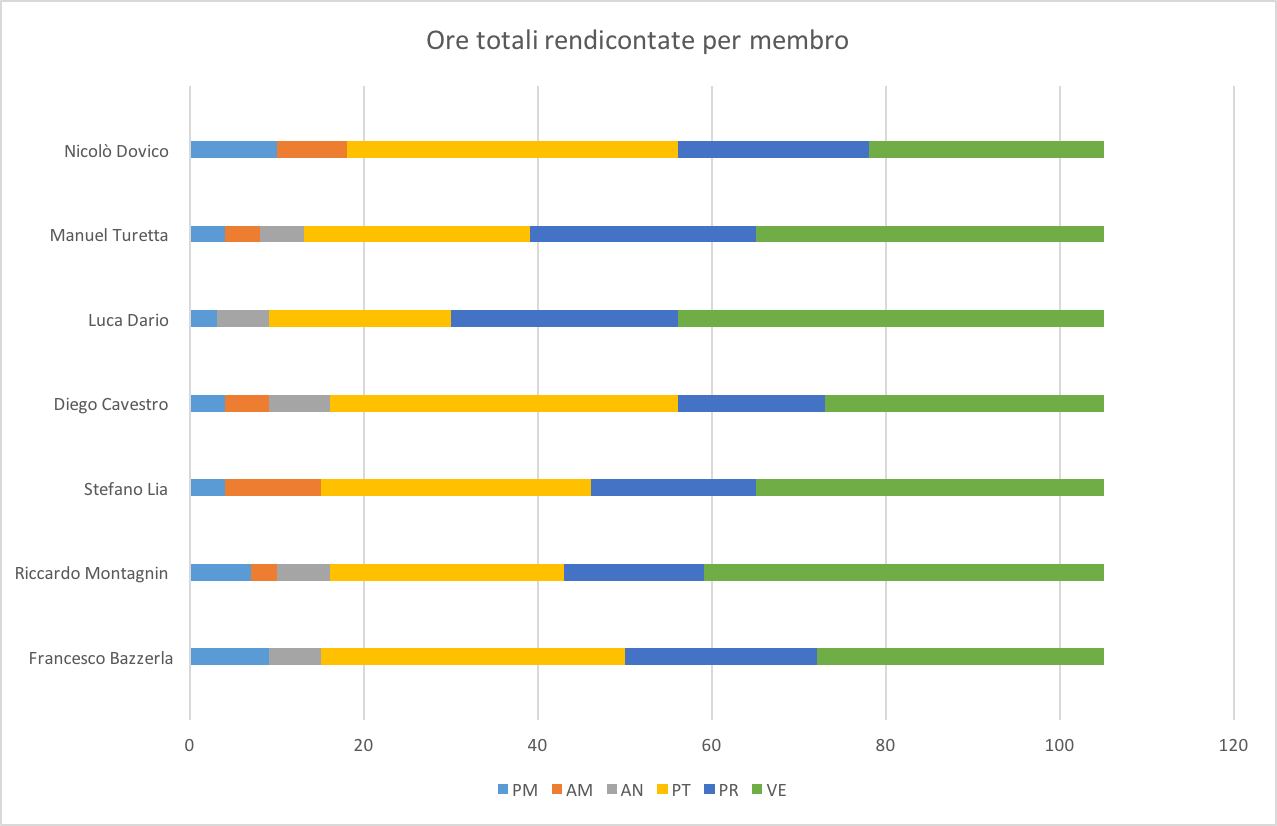
\includegraphics[scale=0.5]{Immagini/Gantt/TOT.png}
	\caption{Diagramma di Gantt, Monolith}
\end{figure}

\subsubsection{\ARM}
Periodo: dal 13/12/2016 all'11/01/2017. \\

L'inizio del periodo di \ARM\ corrisponde all'inizio del progetto. In questo periodo il gruppo deve scegliere un \termine{capitolato} e cominciare a lavorare con il fine ultimo di aggiudicarselo.\\
Ciò comporta la stesura dei seguenti documenti:
 \begin{itemize}
 \item Esterni:
 	\begin{itemize}
 	 \item \AdR
 	 \item \PdP
	 \item \PdQ
 	\end{itemize}
 \item  Interni:
	\begin{itemize}
	\item \SdF
	\item \NdP
	\end{itemize} 
 \end{itemize}
 Il carico di lavoro viene suddiviso principalmente tra i ruoli di \An, \Am, \Ver\ e \Pm.
 Il periodo termina con una milestone esterna, corrispondente alla consegna dei documenti per la \RR.
 
 \begin{figure}[H]
	\centering 
	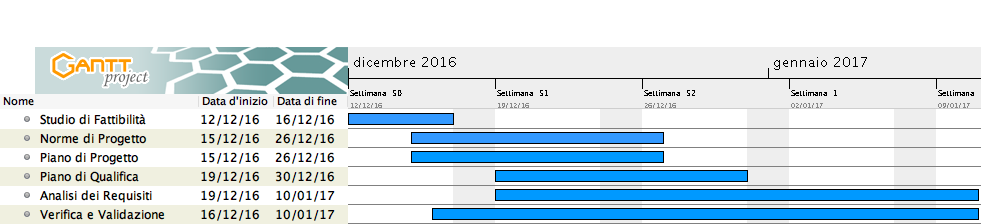
\includegraphics[scale=0.5]{Immagini/Gantt/ARM.png}
	\caption{Diagramma di Gantt, \ARM}
\end{figure}

\subsection{\ARD}
Periodo: dal 12/01/2017 al 03/02/2017 \\

Questo periodo inizia subito dopo la consegna dei documenti per la \RR. Il termine corrisponde ad una \termine{milestone} interna che coincide con l'inizio del periodo successivo, la \PA.\\
Il \termine{gruppo} in questo periodo si impegnerà ad identificare, ampliare e fissare definitivamente i requisiti richiesti per lo svolgimento del progetto.\\
Verranno inoltre effettuate le modifiche necessarie, rilevate in seguito all'esito della \RR\, nei vari documenti.\\
I ruoli coinvolti maggiormente in questo periodo sono: \An, \Am, \Pm\ e \Ver.

\begin{figure}[H]
	\centering 
	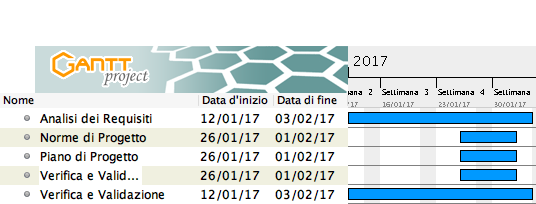
\includegraphics[scale=0.5]{Immagini/Gantt/ARD.png}
	\caption{Diagramma di Gantt, \ARD}
\end{figure}

\subsection{\PA}
Periodo: dal 06/02/2017 al 21/02/2017 \\

Inizia in seguito alla terminazione dell'\ARD\ ed il suo il termine prefissato coincide con una \termine{milestone} interna.
Il \termine{gruppo} si pone l'obbiettivo di eseguire e fissare definitivamente la progettazione del sistema ad alto livello e di redigere il documento \ST.\\
In quest'ultimo documento i \ProgP\ dovranno descrivere, ad alto livello, le scelte progettuali ed il \termine{design-pattern} scelti per la realizzazione dell'architettura generale del \termine{prodotto}. Vengono inoltre incrementati i documenti \NdP, \PdP, \PdQ\ e \Gl.\\
In questo periodo i ruoli maggiormente interessati sono: \Prog, \Pm, \Ver\ e \Am.

 \begin{figure}[H]
	\centering 
	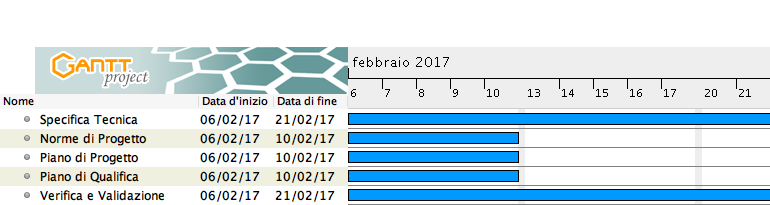
\includegraphics[scale=0.5]{Immagini/Gantt/PA.png}
	\caption{Diagramma di Gantt, \PA}
\end{figure}

\subsection{\PD}
Periodo: dal 22/02/2017 al 06/03/2017\\

Dal seguente periodo lo svolgimento dei passi successivi segue il \termine{Modello Incrementale}, ovvero verranno realizzati prima i requisiti essenziali, poi quelli desiderabili e infine quelli facoltativi per ridurre il rischio di fallimento. 
Inizia in seguito all'approvazione della \PA\ e si conclude entro la consegna del prodotto alla \RQ.
Il gruppo si impegna a terminare la \PD\ almeno delle funzionalità essenziali per il 06/03/2017, che coincide con una \termine{milestone} esterna per la consegna dei documenti della \RP.\\
Il gruppo, ad ogni incremento, si impegna ad intraprendere e completare le seguenti attività:
\begin{itemize}
\item
Redigere o aggiornare il documento \DDP\ in cui i \ProgrP\ e i \ProgP\ devono descrivere il comportamento e le interazioni tra i vari componenti del sistema, basandosi sul documento di \ST.
\item
Incrementare i documenti \NdP, \PdP, \PdQ\ e \Gl.
\end{itemize}
In questo periodo i ruoli maggiormente impegnati sono quelli di \Prog, \Progr, \Pm, \Ver\ e \Am.

 \begin{figure}[H]
	\centering 
	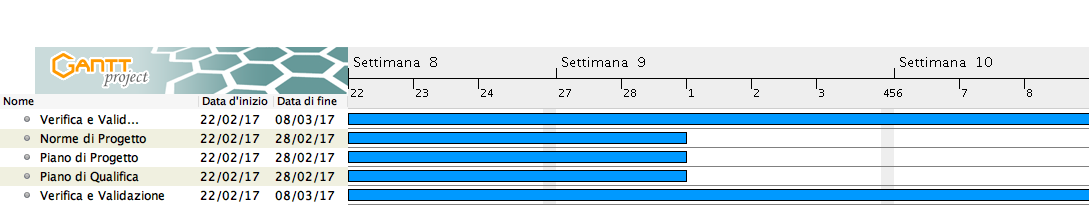
\includegraphics[scale=0.5]{Immagini/Gantt/PD.png}
	\caption{Diagramma di Gantt, \PD}
\end{figure}

\subsubsection{\COD}
Periodo: dal 14/03/2017 all'11/04/2017. \\

Il periodo di \COD\ avviene in concorrenza a quello di \PD ed inizia una volta completata la progettazione dettagliata delle funzionalità essenziali. Essa si conclude con la consegna del prodotto alla \RQ. L'obiettivo finale consiste nel consegnare un prodotto completo, e le attività che ad ogni incremento verranno eseguite a tal fine sono le seguenti:
\begin{itemize}
	\item \COD: I \ProgrP\ devono sviluppare il codice del prodotto software attenendosi il più possibile a quanto scritto dai \ProgP\ nel documento \DDP. L'attività di \COD\ deve essere fatta seguendo, iterativamente, i seguenti passi:
			\begin{itemize}
				\item \termine{Codifica} dell'incremento svolto dai \ProgP.
				\item \termine{Verifica} dell'incremento.
			\end{itemize}
	\item Stesura o ampliamento del \MU: questo documento è destinato all'utilizzatore finale del prodotto che, tramite esso, deve essere in grado di capire le principali funzionalità del sistema e come utilizzarle.
	\item \termine{Verifica} dei documenti, della progettazione e del software prodotto con gli strumenti definiti nelle \NdP.
\end{itemize}
I ruoli maggiormente interessati sono quelli di \Am, \Pm, \Prog, \Progr\ e \Ver.

 \begin{figure}[H]
	\centering 
	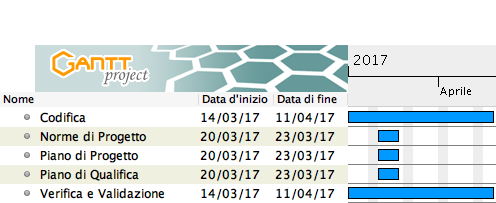
\includegraphics[scale=0.5]{Immagini/Gantt/COD.png}
	\caption{Diagramma di Gantt, \COD}
\end{figure}

\subsubsection{Verifica e Validazione}
Periodo: dal 16/12/2016 al 14/05/2017.\\

Questo periodo, come si può osservare dalla data di inizio, è trasversale a tutti i periodi. Infatti, per garantire ad ogni incremento efficacia ed efficienza del prodotto, le operazioni di \termine{testing}, \termine{verifica} e \termine{validazione} vengono eseguite durante tutto il corso del progetto.\\

\paragraph{\VV}
Periodo: dal 12/04/2017 al 15/05/2017 \\

Al termine della \PD e \COD\ verranno effettuati ed intensificati tutti i test necessari per garantire che il prodotto soddisfi tutti i requisiti dell'\AdR e la correzione di eventuali errori nel codice e/o nei vari documenti.
Le attività prevedono di:
\begin{itemize}
	\item Effettuare dei test di sistema.
	\item Incrementare, correggere o aggiornare i documenti di: \MU, \NdP, \PdP, \PdQ\ e \Gl.
	\item Verificare tutti i documenti sopra citati.
	\item Verificare il corretto funzionamento del prodotto correggendo eventuali errori.
\end{itemize}
In questo periodo i ruoli maggiormente interessati sono quelli di \Ver, \Prog, \Am\ e \Pm.

 \begin{figure}[H]
	\centering 
	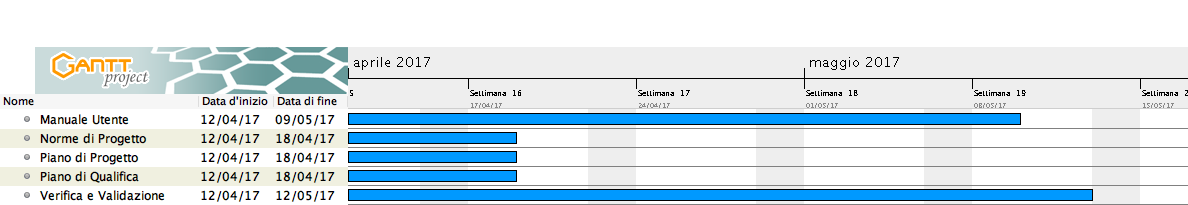
\includegraphics[scale=0.5]{Immagini/Gantt/VV.png}
	\caption{Diagramma di Gantt, \VV}
\end{figure}
\newpage
\section{Preventivo}
In questa sezione vengono presentati i grafici e le tabelle riassuntive per descrivere l'impegno previsto, in ore lavoro, dei diversi ruoli nei sei periodi sopra descritti. Inoltre viene mostrata una tabella riassuntiva al fine di rappresentare l'incidenza di ogni ruolo nell'intero progetto.

\subsection{\ARM}
Questa fase è considerata un investimento del \termine{team} per aggiudicarsi il progetto e per tale motivo non verrà rendicontata nel calcolo del preventivo. \\
Le ore impiegate in questo periodo sono 179 e vengono ripartite in:

\begin{table}[h]
	\begin{center}
		\begin{tabular}{|c|c|}
			\hline
			\textbf{Ruolo}	& \textbf{Ore} \\
			\hline
			\Pm &	20\\
			\hline
			\Am	&	19\\
			\hline
			\An		&	75\\
			\hline
			\Ver	&	65\\
			\hline
		\end{tabular}
	\end{center}
	\caption{Ore per ruolo, \ARM}
\end{table}

\begin{figure}[H]
	\centering 
	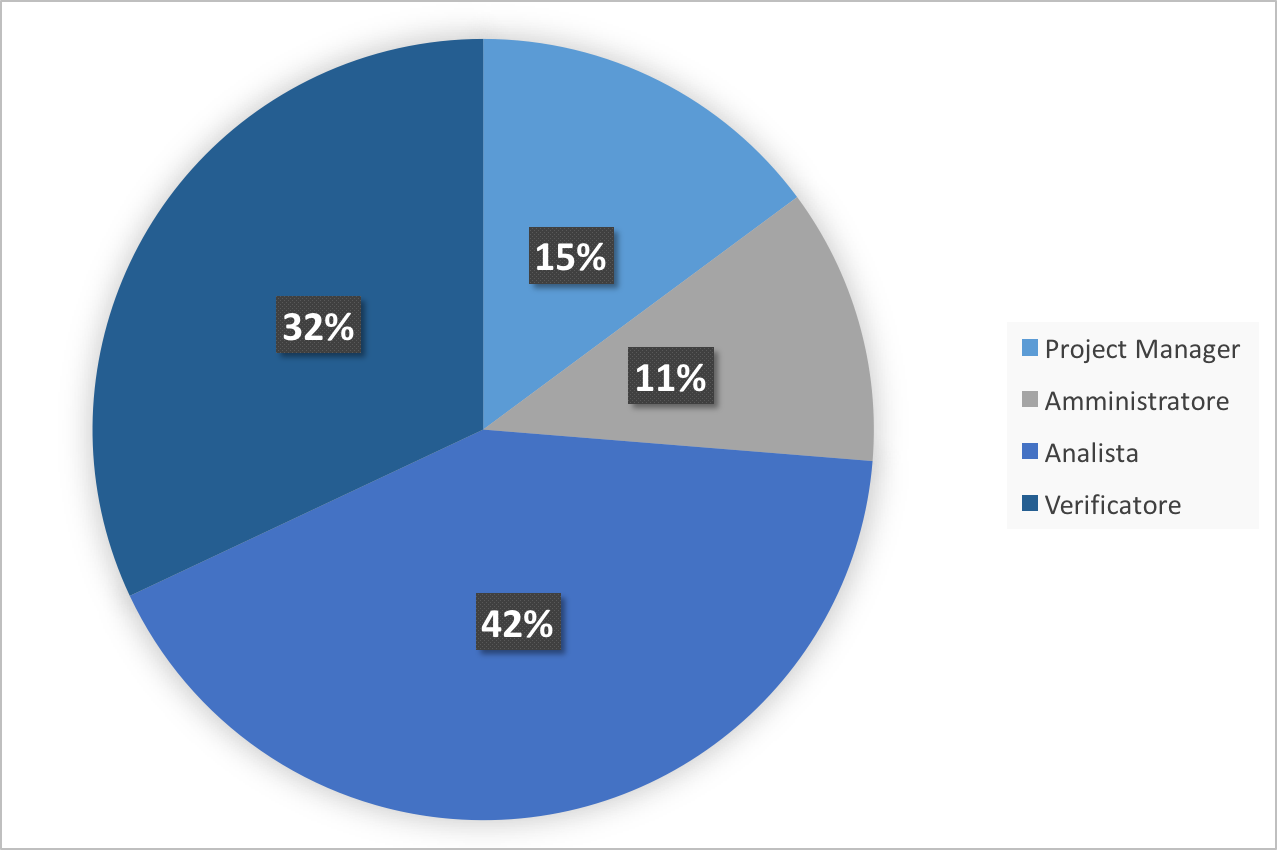
\includegraphics[scale=0.7]{Immagini/GraficiTorte/ARM.png}
	\caption{Ore per ruolo, \ARM}
\end{figure}

\newpage
\subsection{\ARD}
Le ore impiegate in questo periodo sono 50 e vengono ripartite in:

\begin{table}[h]
	\begin{center}
		\begin{tabular}{|c|c|}
			\hline
			\textbf{Ruolo}	& \textbf{Ore} \\
			\hline
			\Pm &	3\\
			\hline
			\Am	&	3\\
			\hline
			\An		&	30\\
			\hline
			\Ver	&	14\\
			\hline
		\end{tabular}
	\end{center}
	\caption{Ore per ruolo, \ARD}
\end{table}

\begin{figure}[H]
	\centering 
	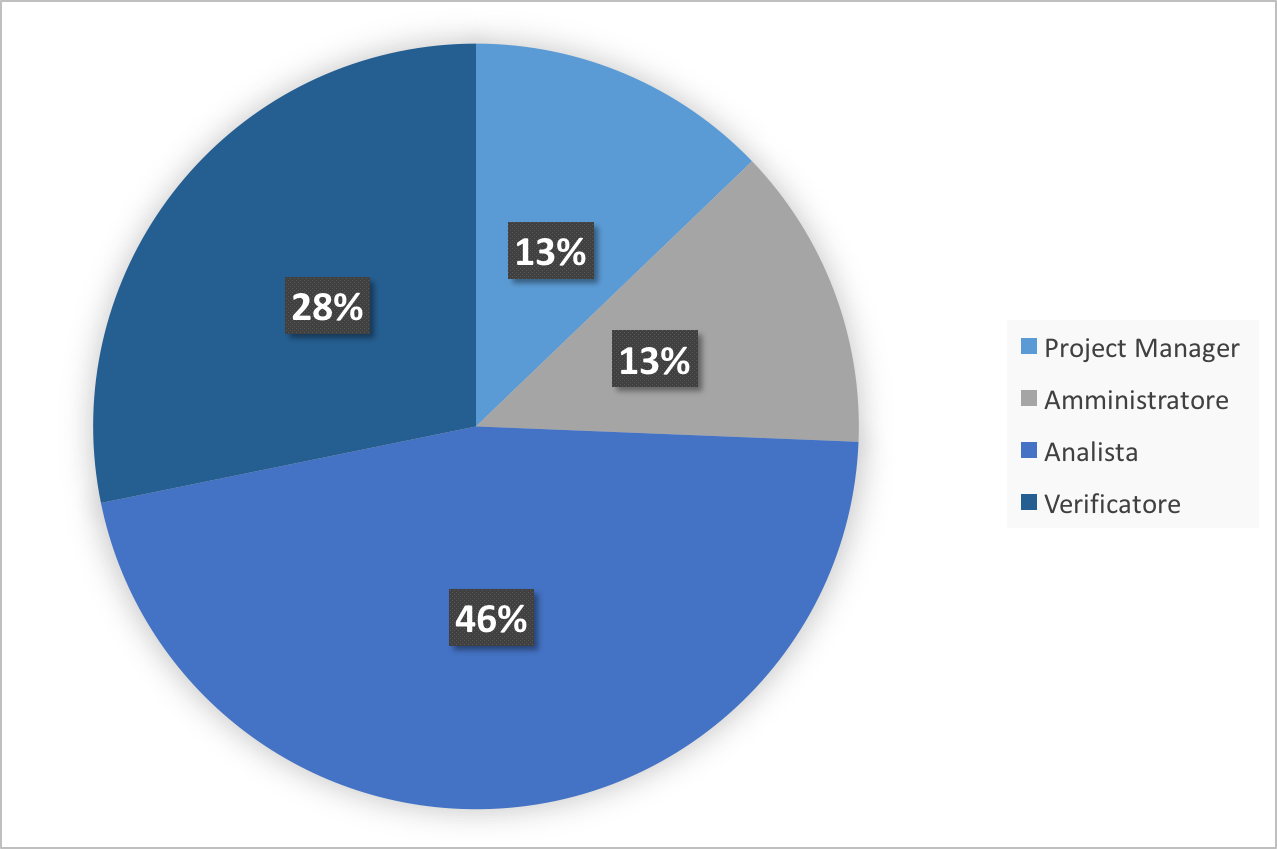
\includegraphics[scale=0.7]{Immagini/GraficiTorte/ARD.png}
	\caption{Ore per ruolo, \ARD}
\end{figure}
\newpage
\subsection{\PA}
Le ore totali impiegate in questo periodo sono 198 e vengono ripartite in:

\begin{table}[h]
	\begin{center}
		\begin{tabular}{|c|c|}
			\hline
			\textbf{Ruolo}	& \textbf{Ore} \\
			\hline
			\Pm &	6\\
			\hline
			\Am	& 7\\
			\hline
			\Prog & 120\\
			\hline
			\Ver	&	65\\
			\hline
		\end{tabular}
	\end{center}
	\caption{Ore per ruolo, \PA}
\end{table}

\begin{figure}[H]
	\centering 
	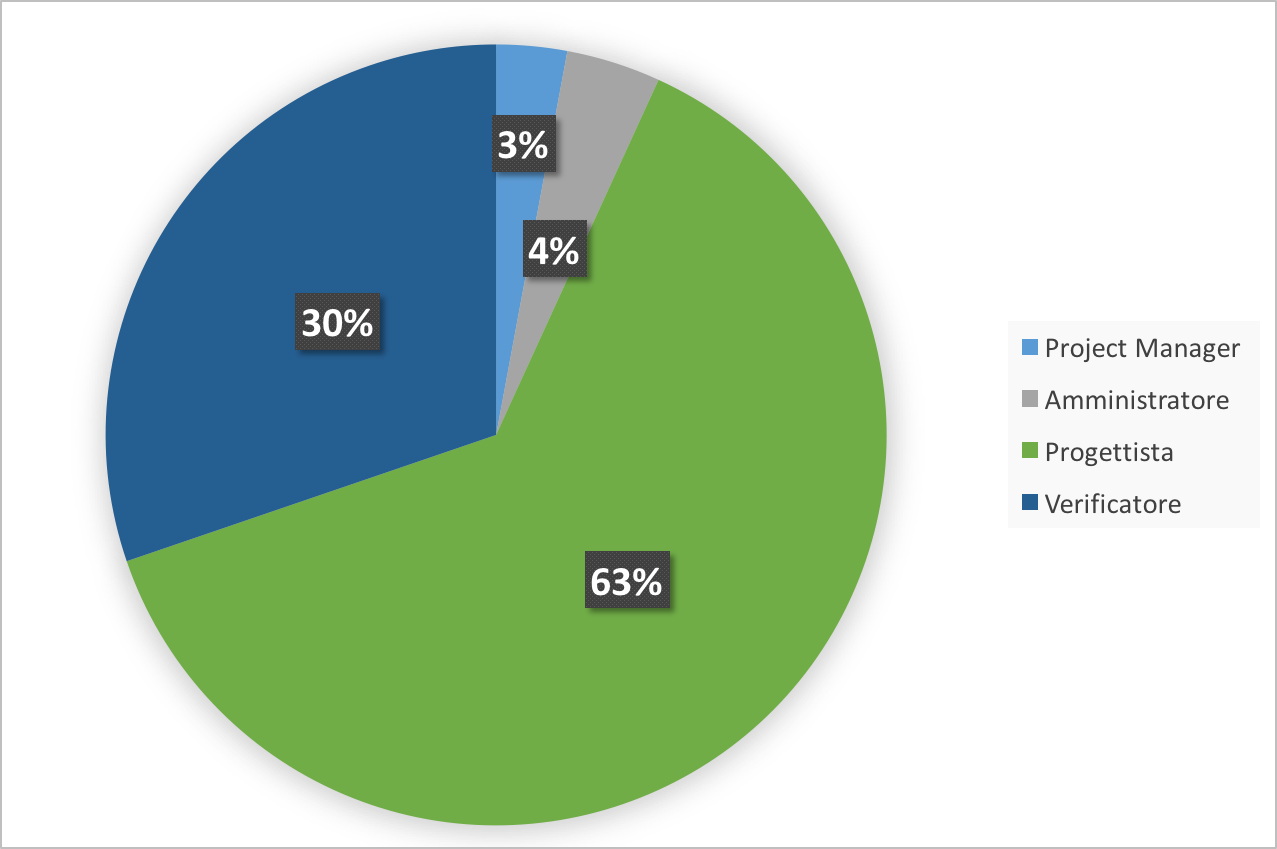
\includegraphics[scale=0.7]{Immagini/GraficiTorte/PA.png}
	\caption{Ore per ruolo, \PA}
\end{figure}

\newpage
\subsection{\PD\ e \COD}
Le ore totali impiegate in questo periodo sono 478 e vengono ripartite in:

\begin{table}[h]
	\begin{center}
		\begin{tabular}{|c|c|}
			\hline
			\textbf{Ruolo}	& \textbf{Ore} \\
			\hline
			\Pm &	20\\
			\hline
			\Am	&	12\\
			\hline
			\Prog	&	107\\
			\hline
			\Progr	&	200\\
			\hline
			\Ver	&	139\\
			\hline
		\end{tabular}
	\end{center}
	\caption{Ore per ruolo, \PD\ e \COD}
\end{table}

\begin{figure}[H]
	\centering 
	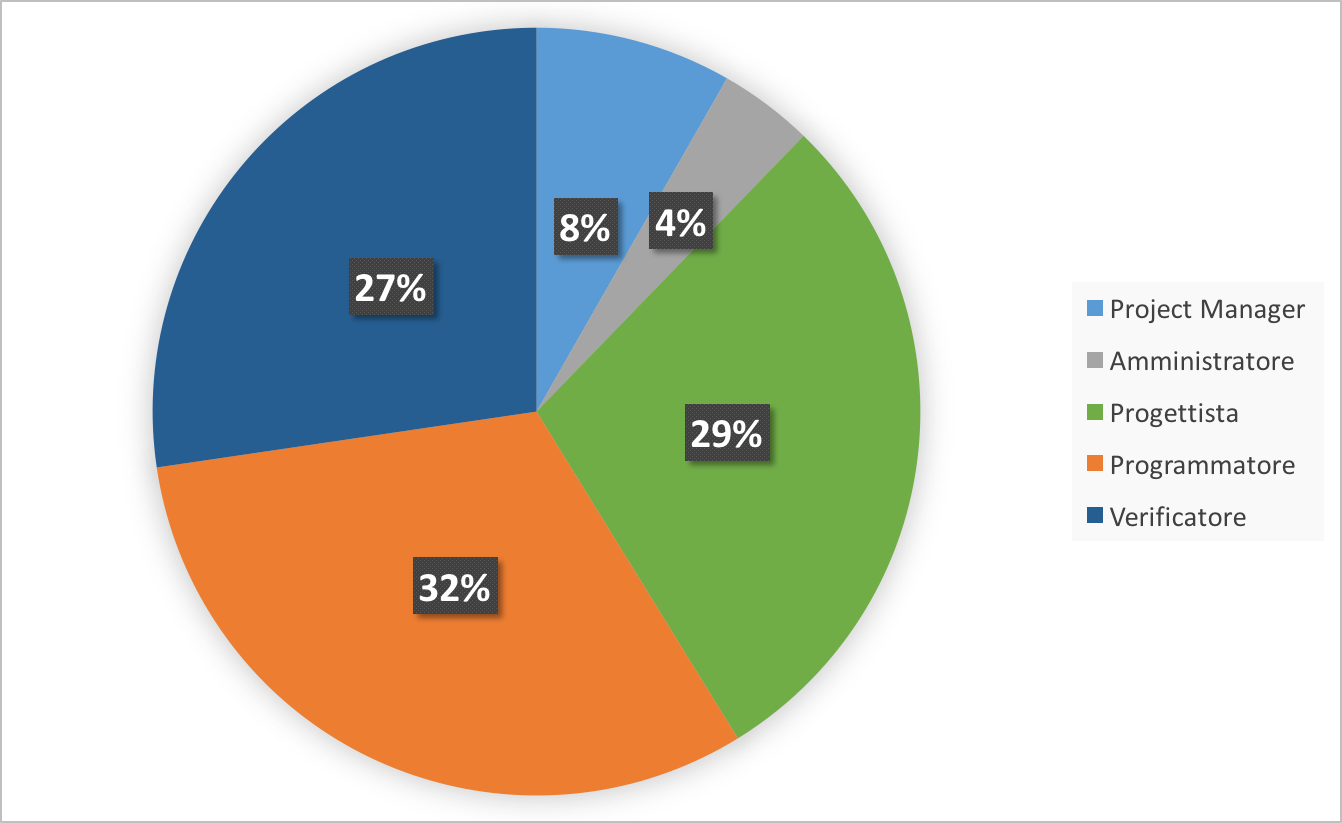
\includegraphics[scale=0.7]{Immagini/GraficiTorte/PDCOD.png}
	\caption{Ore per ruolo, \PD\ e \COD}
\end{figure}

\newpage
Fino alla \RP\ sono state pianificate 121 delle ore descritte in precedenza suddivise come segue:

\begin{table}[h]
	\begin{center}
		\begin{tabular}{|c|c|}
			\hline
			\textbf{Ruolo}	& \textbf{Ore} \\
			\hline
			\Pm &	7\\
			\hline
			\Am	&	7\\
			\hline
			\Prog	&	65\\
			\hline
			\Ver	&	42\\
			\hline
		\end{tabular}
	\end{center}
	\caption{Ore per ruolo, \PD\ e \COD\ fino a \RP}
\end{table}

\begin{figure}[H]
	\centering 
	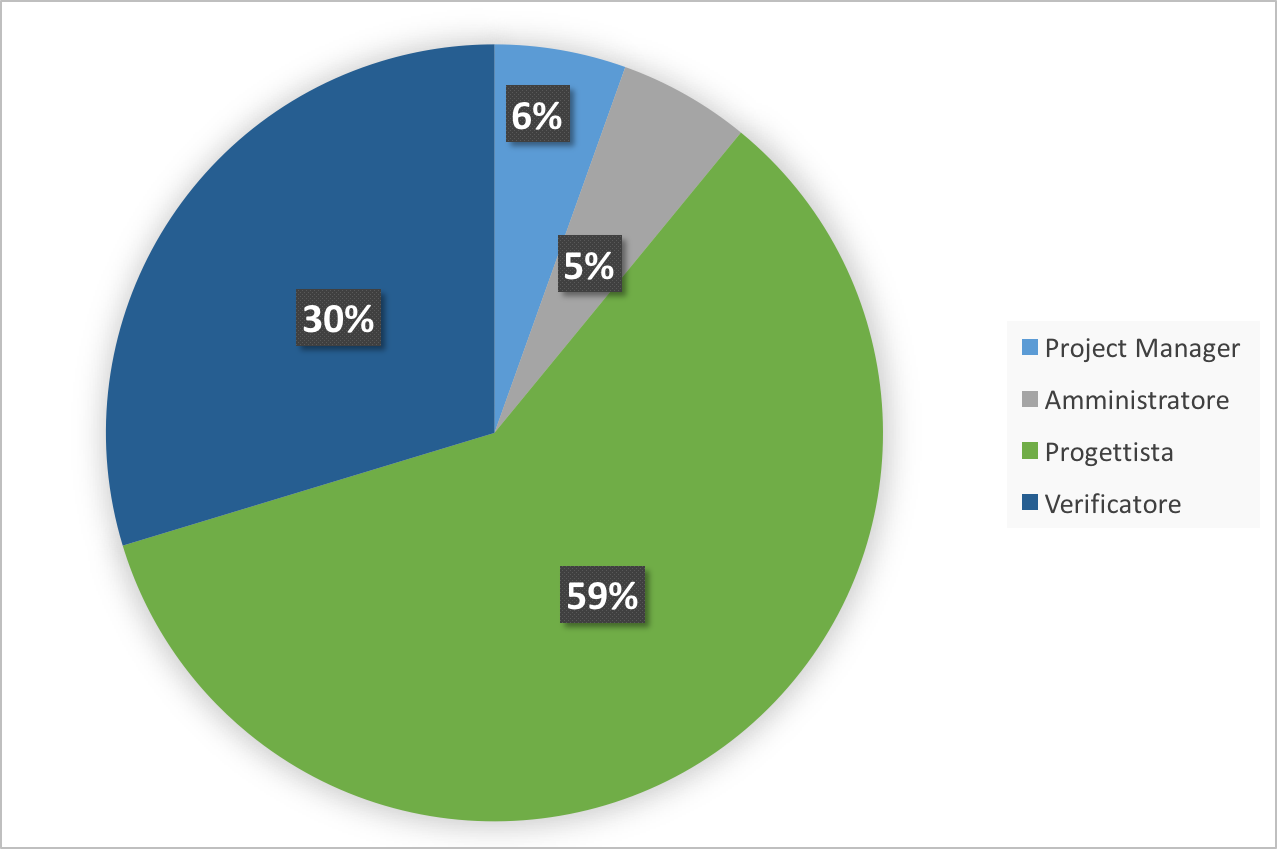
\includegraphics[scale=0.7]{Immagini/GraficiTorte/PD.png}
	\caption{Ore per ruolo, \PD\ e \COD\ fino a \RP}
\end{figure}

\newpage
Mentre dalla \RP\ fino al termine coincidente con la consegna per la \RQ\ le 357 ore rimanenti sono suddivise come segue:

\begin{table}[h]
	\begin{center}
		\begin{tabular}{|c|c|}
			\hline
			\textbf{Ruolo}	& \textbf{Ore} \\
			\hline
			\Pm &	13\\
			\hline
			\Am	&	5\\
			\hline
			\Prog	&	42\\
			\hline
			\Progr	&	200\\
			\hline
			\Ver	&	97\\
			\hline
		\end{tabular}
	\end{center}
	\caption{Ore per ruolo, \PD\ e \COD\ da \RP\ fino a \RQ}
\end{table}

\begin{figure}[H]
	\centering 
	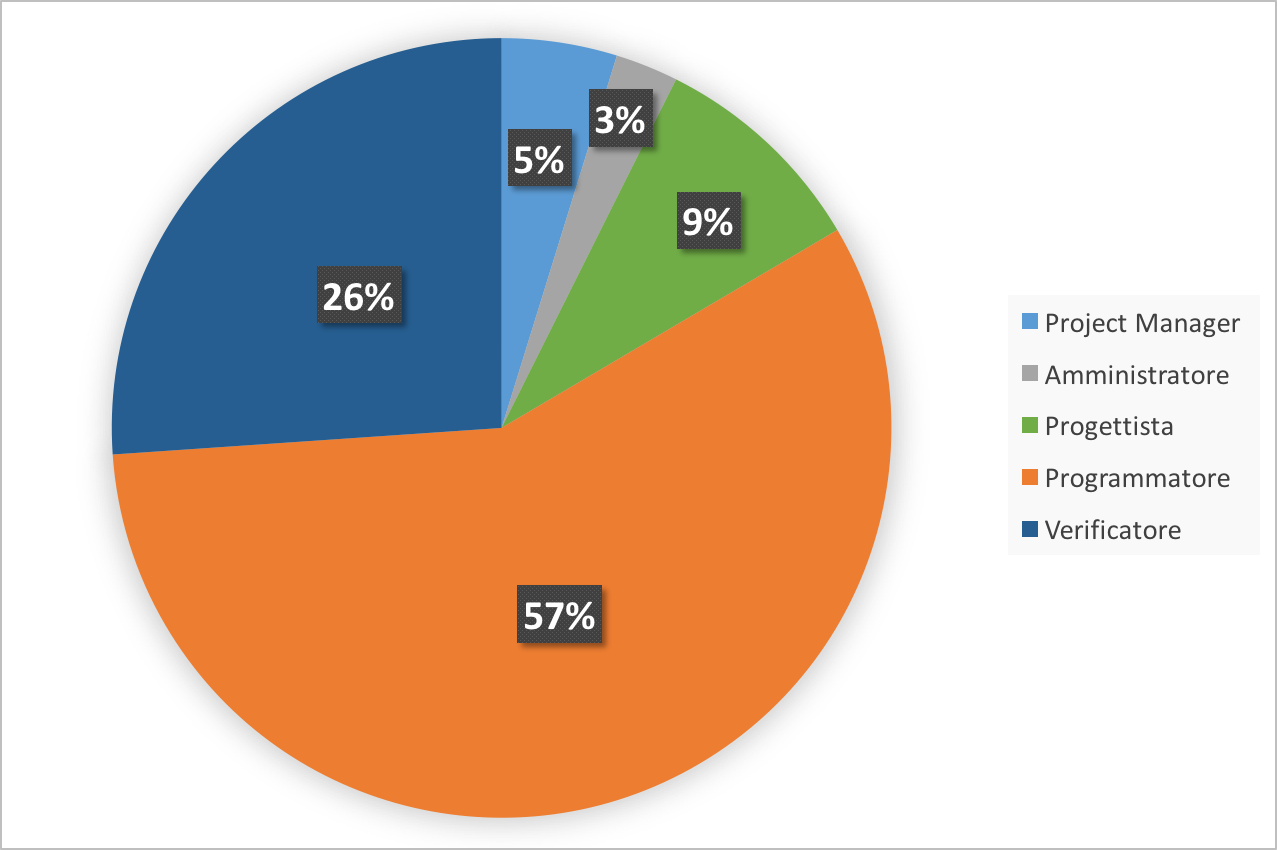
\includegraphics[scale=0.7]{Immagini/GraficiTorte/COD.png}
	\caption{Ore per ruolo, \PD\ e \COD\ da \RP\ fino a \RQ}
\end{figure}

Le ore di questo periodo di \PD\ e \COD\ includono anche 70 ore di autoapprendimento. Infatti, dato il verificarsi del rischio tecnologico relativo alla difficile comprensione di alcune tecnologie, in particolare la difficile comprensione della documentazione della piattaforma \termine{Rocket.chat}, sono state previste ulteriori ore di autoapprendimento per i ruoli di \Progr\ e \Ver\ suddivise come segue:

\begin{table}[h]
	\begin{center}
		\begin{tabular}{|c|c|}
			\hline
			\textbf{Ruolo}	& \textbf{Ore} \\
			\hline
			\Progr	&	56\\
			\hline
			\Ver	&	14\\
			\hline
		\end{tabular}
	\end{center}
	\caption{Ore di autoapprendimento per ruolo, \PD\ e \COD\ da \RP\ fino a \RQ}
\end{table}

Le ore di autoapprendimento, come le ore di investimento iniziale, non verranno rendicontate nel calcolo del preventivo.

\newpage
\subsection{\VV}
Le ore totali in questo periodo sono 78 e vengono ripartite in:

\begin{table}[h]
	\begin{center}
		\begin{tabular}{|c|c|}
			\hline
			\textbf{Ruolo}	& \textbf{Ore} \\
			\hline
			\Pm &	8\\
			\hline
			\Am	&	3\\
			\hline
			\Prog		&	6\\
			\hline
			\Progr & 8\\
			\hline
			\Ver	&	53\\
			\hline
		\end{tabular}
	\end{center}
	\caption{Ore per ruolo, \VV}
\end{table}

\begin{figure}[H]
	\centering 
	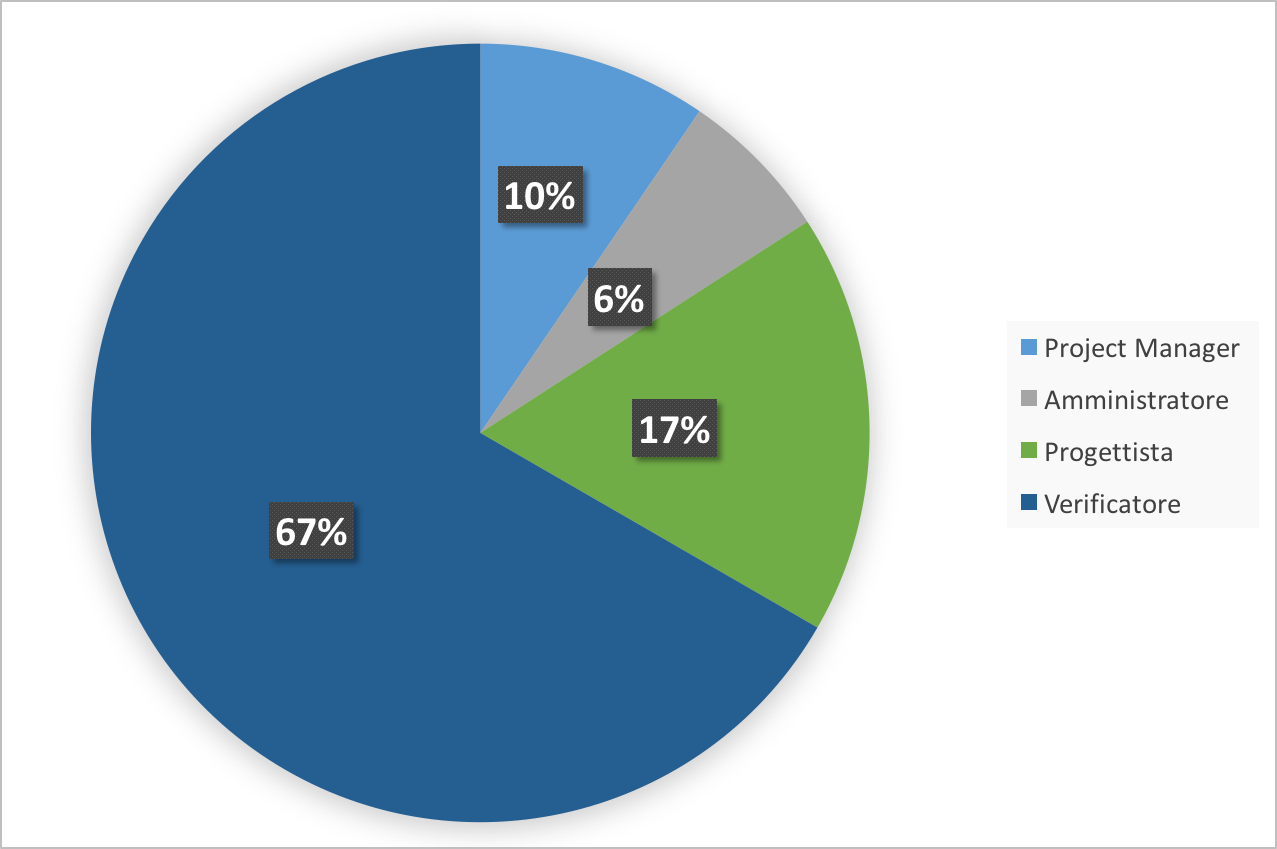
\includegraphics[scale=0.7]{Immagini/GraficiTorte/VV.png}
	\caption{Ore per ruolo, \VV}
\end{figure}
\newpage
\subsection{Quadro riassuntivo}
Le ore totali del progetto sono 983, di cui 734 remunerabili, così ripartite:

\begin{table}[h]
	\begin{center}
		\begin{tabular}{|c|c|c|}
			\hline
			\textbf{Ruolo}	& \textbf{Ore totali} & \textbf{Ore remunerabili} \\
			\hline
			\Pm &	57	&	37	\\
			\hline
			\Am	&	44	&	25	\\
			\hline
			\An		&	105	&	30	\\
			\hline
			\Prog		&	233	&	233	\\
			\hline
			\Progr	&	208	&	152	\\
			\hline
			\Ver	&	336	&	257	\\
			\hline
		\end{tabular}
	\end{center}
	\caption{Ore per ruolo, Quadro riassuntivo}
\end{table}

\begin{figure}[H]
	\centering 
	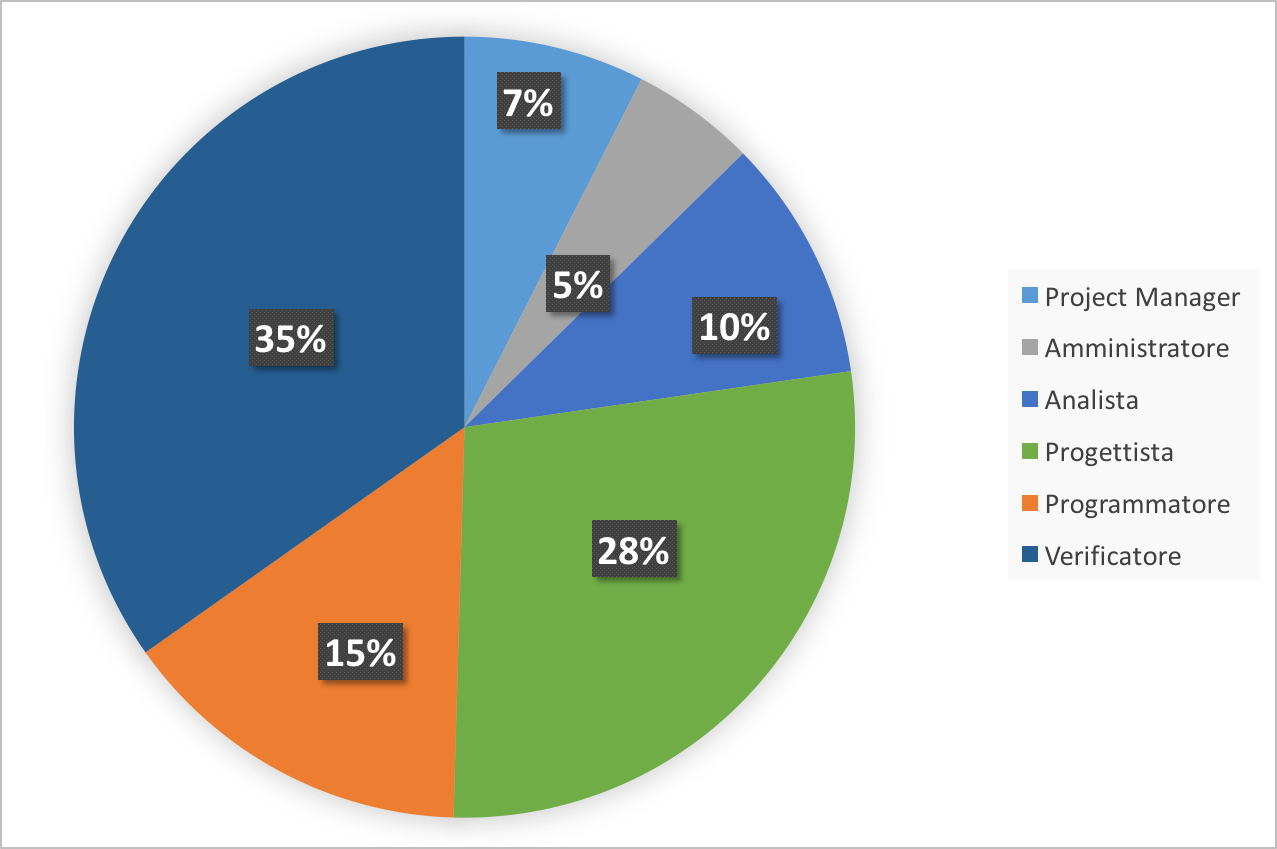
\includegraphics[scale=0.7]{Immagini/GraficiTorte/TOT.png}
	\caption{Ore totali per ruolo}
\end{figure}
\newpage
\section{Suddivisione del lavoro}
I componenti del gruppo dovranno rivestire ciascuno, almeno una volta, tutti i ruoli specificati nell'\textit{organigramma\ped{G}}.
Durante le varie fasi ogni componente può ricoprire più ruoli, anche contemporaneamente, purchè non si presentino dei conflitti di interesse tra le attività svolte. Ad esempio un componente non potrà essere \textit{\Ver} del codice scritto da egli stesso.
\paragraph{Legenda}
\begin{itemize}
\item\textbf{PM:} \Pm
\item\textbf{AM:} \Am
\item\textbf{AN:} \An
\item\textbf{PT:} \Prog
\item\textbf{PR:} \Progr
\item\textbf{VE:} \Ver
\end{itemize}
\subsection{\ARM}

Nell'attività di \ARM\ ciascun componente dovrà rivestire i seguenti ruoli:


\begin{table}[h]
	\begin{center}
		\begin{tabular}{|c|c|c|c|c|c|c|c|}
			\hline
			\textbf{Nominativo} & \multicolumn{6}{c|}{\textbf{Ore per ruolo}} & \textbf{Ore totali} \\
					& PM & AM & AN & PT & PR & VE & \\
			\hline
			\FB		&	 &	5 &	10 &  	&	 & 10 &	25	\\
			\hline
			\RM		& 11 &	  &	4  & 	&	 & 10 &	25	\\
			\hline
			\SL		& 8  & 6  &	11 &	&	 &	  &	25	\\
			\hline
			\DC		&	 & 1  &	8  &	&	 & 16 &	25	\\
			\hline
			\LD 	& 7	 & 2  &	10 &	&	 & 6  &	25	\\
			\hline
			\MT		& 	 &    &	11 &	&	 & 14 &	25	\\
			\hline
			\ND 	&	 & 6  &	19 &	&	 &	  & 25	\\
			\hline
		\end{tabular}
	\end{center}
	\caption{Costo per ruolo, \ARM}
\end{table}

\begin{figure}[H]
	\centering 
	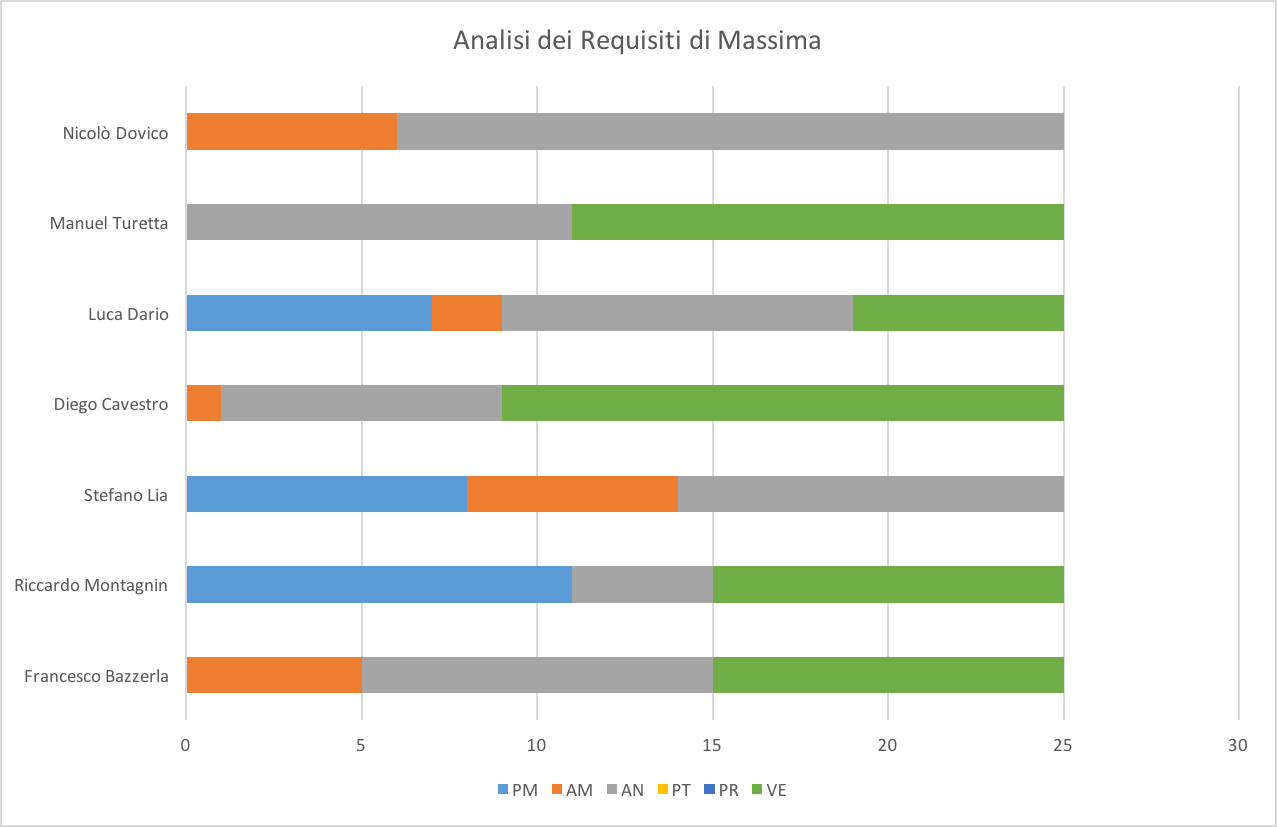
\includegraphics[scale=0.7]{Immagini/GraficiPianoLavoro/ARM.png}
	\caption{Incidenza ore per membro, \ARM}
\end{figure}

\newpage
\subsection{\ARD}
Nell'attività di \ARD ciascun componente dovrà rivestire i seguenti ruoli:

\begin{table}[h]
	\begin{center}
		\begin{tabular}{|c|c|c|c|c|c|c|c|}
			\hline
			\textbf{Nominativo} & \multicolumn{6}{c|}{\textbf{Ore per ruolo}} & \textbf{Ore totali} \\
					& PM & AM & AN & PT & PR & VE & \\
			\hline
			\FB		& 	 &	  &	3  &	&	 & 3  &	6 \\
			\hline
			\RM		&	 & 2  &	3  &	&	 &	  &	5	\\
			\hline
			\SL		& 2	 &	  &	   &	&	 & 4  &	6	\\
			\hline
			\DC		&	 &	  &	6  &	&	 & 	  &	6	\\
			\hline
			\LD 	&	 &	  &	4  &	&	 & 1  &	5	\\
			\hline
			\MT		& 	 & 3  &	2  &	&	 &	  &	5	\\
			\hline
			\ND 	& 3	 &	  &	   &	&	 & 3  &	6	\\
			\hline
		\end{tabular}
	\end{center}
	\caption{Costo per ruolo, \ARD}
\end{table}

\begin{figure}[H]
	\centering 
	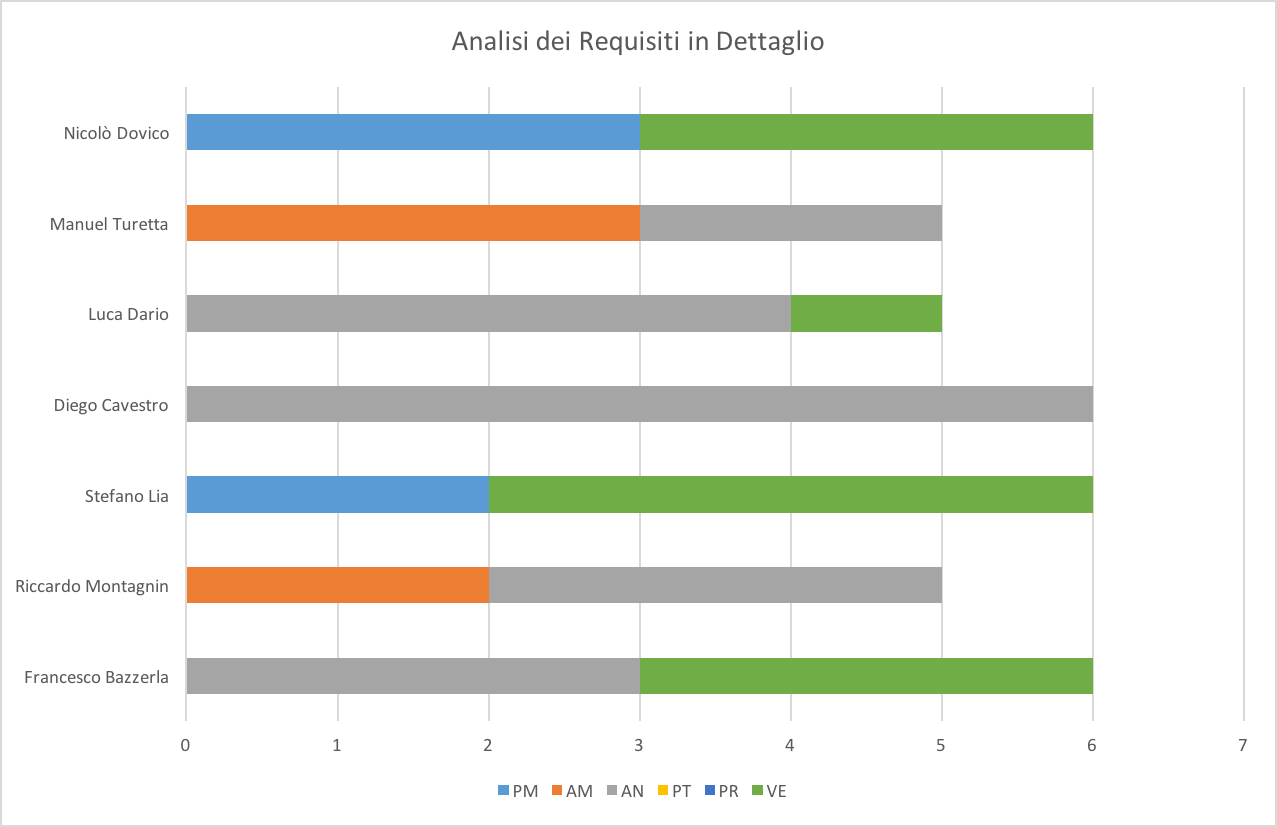
\includegraphics[scale=0.7]{Immagini/GraficiPianoLavoro/ARD.png}
	\caption{Incidenza ore per membro, \ARD}
\end{figure}

\newpage
\subsection{\PA}
Nel periodo di \PA ciascun componente del gruppo dovrà rivestire i seguenti ruoli:

\begin{table}[h]
	\begin{center}
		\begin{tabular}{|c|c|c|c|c|c|c|c|}
			\hline
			\textbf{Nominativo} & \multicolumn{6}{c|}{\textbf{Ore per ruolo}} & \textbf{Ore totali} \\
					& PM & AM & AN & PT & PR & VE & \\
			\hline
			\FB		&	 &	  &	   & 23	&	 & 6  &	29	\\
			\hline
			\RM		&	 & 2  &	   & 14	&  	 & 14 & 30	\\
			\hline
			\SL		&	 &	  &	   & 18	&	 & 11 &	29	\\
			\hline
			\DC		&	 & 6  &	   & 23	&	 & 	  &	29	\\
			\hline
			\LD 	& 3	 &	  &	   & 14	&	 & 12 &	29	\\
			\hline
			\MT		& 3	 &	  &	   & 14	&	 & 13 &	30	\\
			\hline
			\ND 	&	 &	  &	   & 23	&	 & 6  & 29	\\
			\hline
		\end{tabular}
	\end{center}
	\caption{Costo per ruolo, \PA}
\end{table}

\begin{figure}[H]
	\centering 
	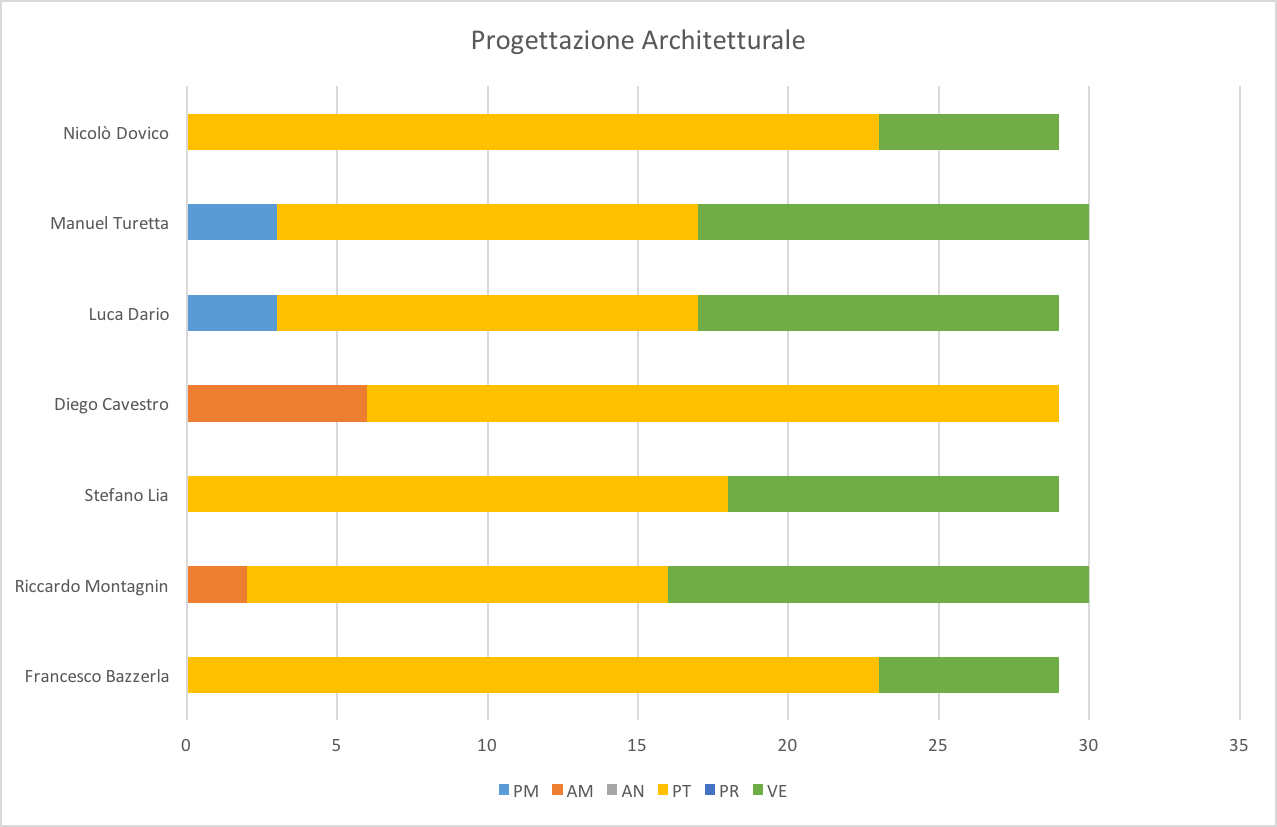
\includegraphics[scale=0.7]{Immagini/GraficiPianoLavoro/PA.png}
	\caption{Incidenza ore per membro, \PA}
\end{figure}

\newpage
\subsection{\PD}
Nel periodo di \PD ciascun componente del gruppo dovrà rivestire i seguenti ruoli:

\begin{table}[h]
	\begin{center}
		\begin{tabular}{|c|c|c|c|c|c|c|c|}
			\hline
			\textbf{Nominativo} & \multicolumn{6}{c|}{\textbf{Ore per ruolo}} & \textbf{Ore totali} \\
					& PM & AM & AN & PT & PR & VE & \\
			\hline
			\FB		& 4  &	  &	   & 7	&	 & 7  &	18	\\
			\hline
			\RM		&	 &	  &	   & 8	&	 & 10 & 18	\\
			\hline
			\SL		&	 & 5  &	   & 5	&	 & 8  &	18	\\
			\hline
			\DC		& 3	 &	  &	   & 16	&	 & 	  &	19	\\
			\hline
			\LD 	&	 &	  &	   & 12	&	 & 7  &	19	\\
			\hline
			\MT		& 	 & 	  &	   & 12	&	 & 6  &	18	\\
			\hline
			\ND 	&	 & 2  &	   & 16	&	 &	  & 18	\\
			\hline
		\end{tabular}
	\end{center}
	\caption{Costo per ruolo, \PD}
\end{table}

\begin{figure}[H]
	\centering 
	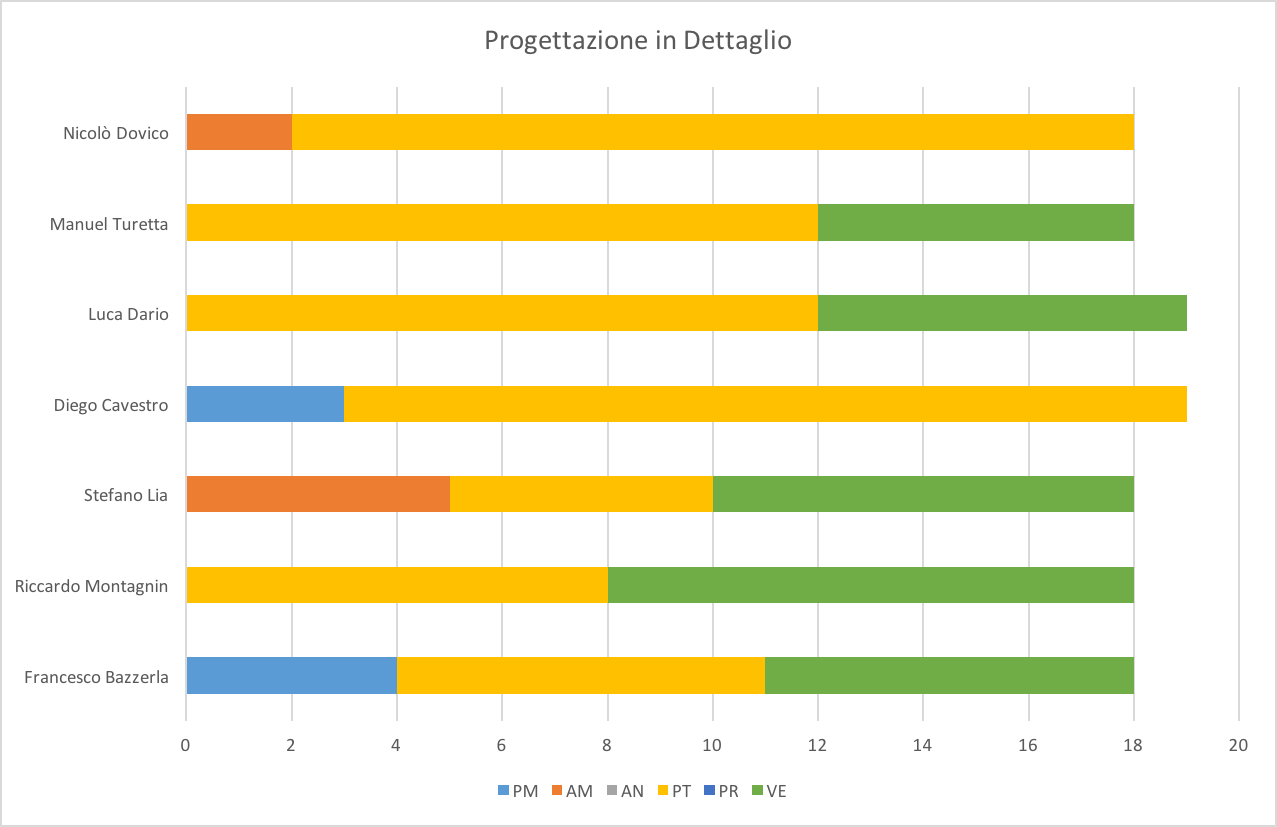
\includegraphics[scale=0.7]{Immagini/GraficiPianoLavoro/PD.png}
	\caption{Incidenza ore per membro, \PD}
\end{figure}

\newpage
\subsection{\COD}
Nel periodo di \COD ciascun componente del gruppo dovrà rivestire i seguenti ruoli:

\begin{table}[h]
	\begin{center}
		\begin{tabular}{|c|c|c|c|c|c|c|c|}
			\hline
			\textbf{Nominativo} & \multicolumn{6}{c|}{\textbf{Ore per ruolo}} & \textbf{Ore totali} \\
					& PM & AM & AN & PT & PR & VE & \\
			\hline
			\FB		&	 &	  &	   & 11	& 22 &	  &	33	\\
			\hline
			\RM		&	 &	  &	   & 	& 16 & 17 & 33	\\
			\hline
			\SL		& 2  &	  &	   & 10	& 21 &    &	33	\\
			\hline
			\DC		&	 &	  &	   &	& 7	 & 25 &	32	\\
			\hline
			\LD 	&	 &	  &	   &	& 23 & 10 &	33	\\
			\hline
			\MT		& 	 & 2  &	   &	& 23 & 8  &	33	\\
			\hline
			\ND 	& 9	 & 4  &	   &	& 20 &    & 33	\\
			\hline
		\end{tabular}
	\end{center}
	\caption{Costo per ruolo, \COD}
\end{table}

\begin{figure}[H]
	\centering 
	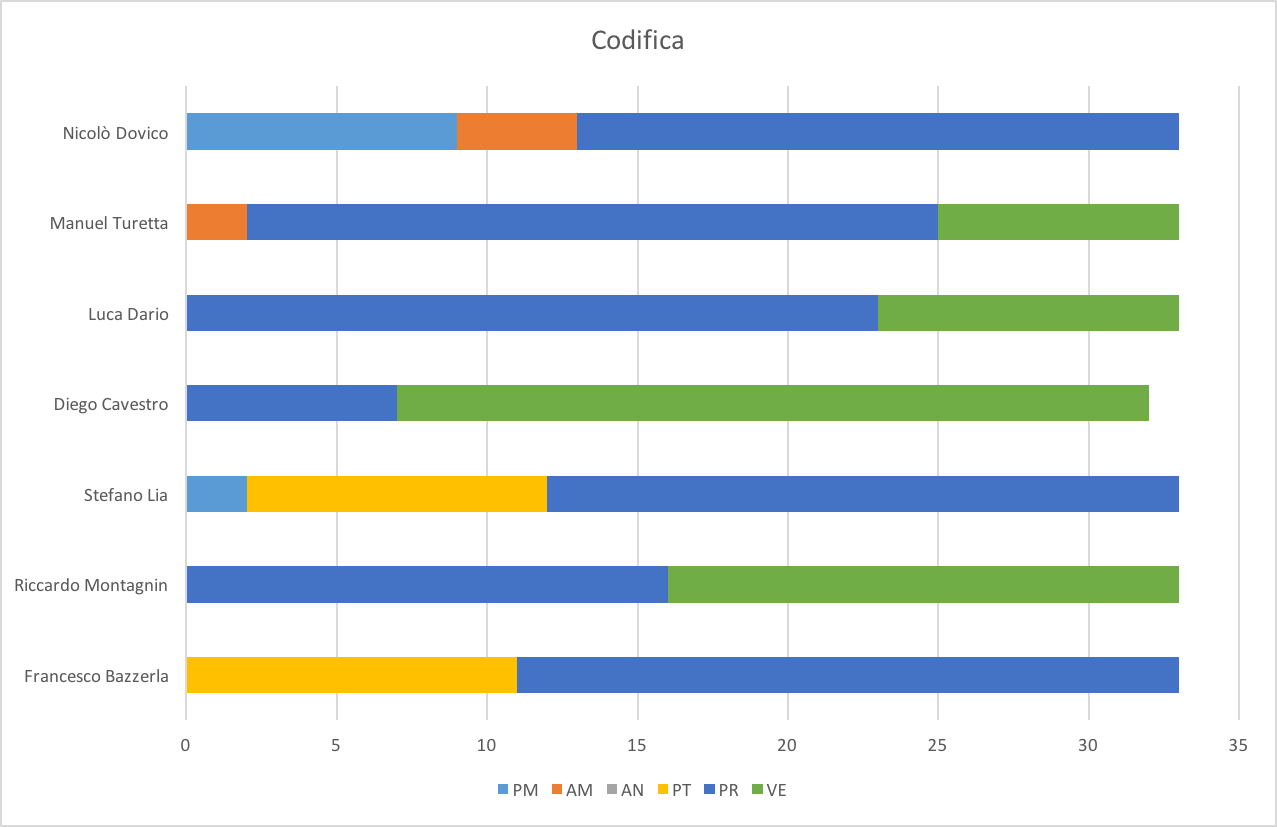
\includegraphics[scale=0.7]{Immagini/GraficiPianoLavoro/COD.png}
	\caption{Incidenza ore per membro, \COD}
\end{figure}

\newpage
\subsection{\VV}
Nel periodo di \VV{} ciascun componente del gruppo dovrà rivestire i seguenti ruoli:

\begin{table}[h]
	\begin{center}
		\begin{tabular}{|c|c|c|c|c|c|c|c|}
			\hline
			\textbf{Nominativo} & \multicolumn{6}{c|}{\textbf{Ore per ruolo}} & \textbf{Ore totali} \\
					& PM & AM & AN & PT & PR & VE & \\
			\hline
			\FB		& 6  &	  &	   &	&	 & 12 &	18	\\
			\hline
			\RM		& 6	 &	  &	   &	&	 & 12 & 18	\\
			\hline
			\SL		&	 & 6  &	   &	&	 & 12 &	18	\\
			\hline
			\DC		&	 &	  &	   & 6  &	 & 12 &	18	\\
			\hline
			\LD 	&	 &	  &	   & 6	&	 & 12 &	18	\\
			\hline
			\MT		& 	 &	  &	   & 6	&	 & 12 &	18	\\
			\hline
			\ND 	&	 & 2  &	   & 4	&	 & 12 & 18	\\
			\hline
		\end{tabular}
	\end{center}
	\caption{Costo per ruolo, \VV}
\end{table}

\begin{figure}[H]
	\centering 
	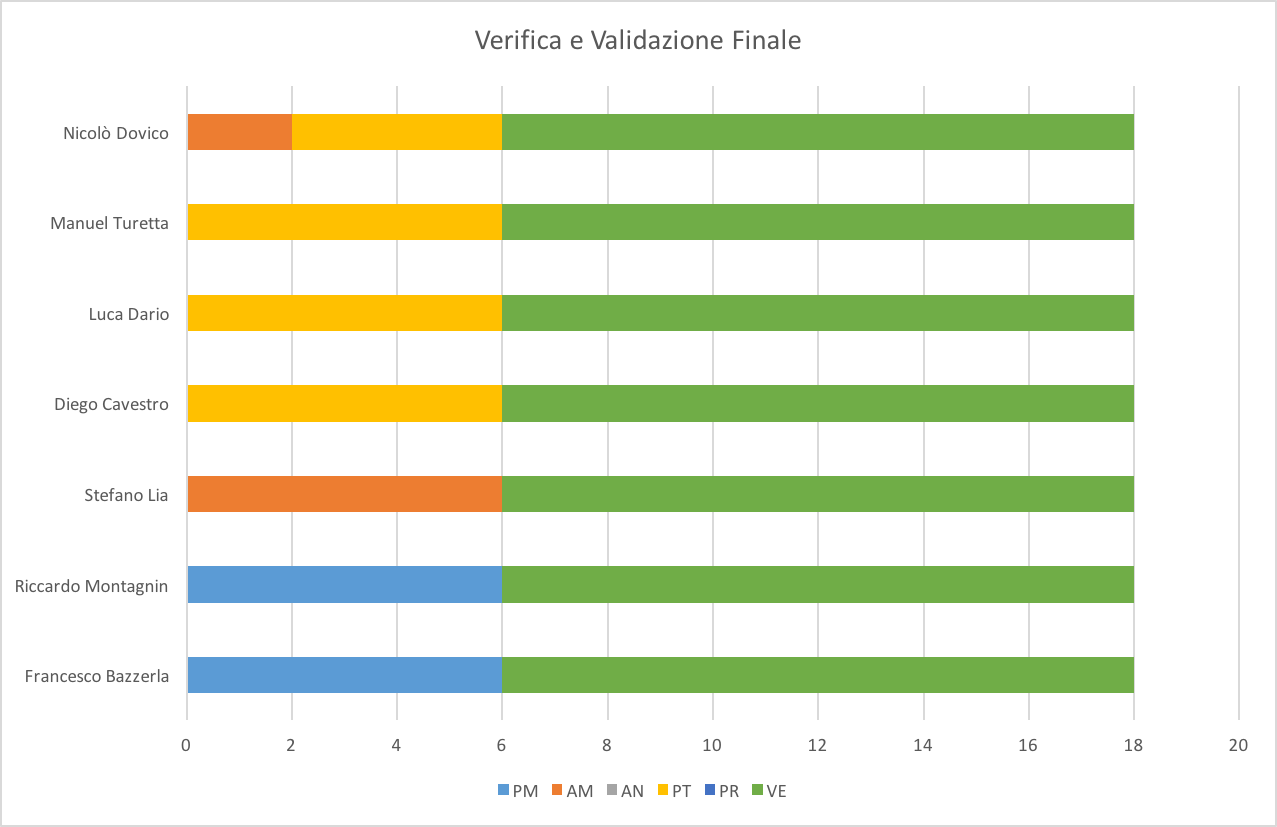
\includegraphics[scale=0.7]{Immagini/GraficiPianoLavoro/VV.png}
	\caption{Incidenza ore per membro, \VV}
\end{figure}

\newpage
\subsection{Totali}
La tabella seguente illustra le ore totali che ogni componente dedicherà per il progetto, mettendo in evidenza anche quelle che verranno poi rendicontate.
\begin{table}[h]
	\begin{center}
		\begin{tabular}{|c|c|c|c|c|c|c|c|c|}
			\hline
			\multirow{2}{*} {\textbf{Nominativo}} & & \multicolumn{6}{c|}{\textbf{Ore per ruolo}} & \multirow{2}{*}{\textbf{Ore totali}} \\
			& & PM & AM & AN & PT & PR & VE & \\
			\hline
			\multirow{2}{*}{\FB}		&	Rendicontate	&	10	&	0	&	3	&	41	&	22	& 28 	&	104	\\
			\cline{2-9}
			&	Totali			&	10	& 5	&	13	&	41	&	22	& 38 &	129	\\
			\hline
			\multirow{2}{*}{\RM}	&	Rendicontate	&	6 &	4	&	3	&	22	&	16	&  53	&	104	\\
			\cline{2-9}
			&	Totali			&	17	&	4	&	7	&	22	&	16	& 	63	&	129	\\
			\hline
			\multirow{2}{*}{\SL}	&	Rendicontate	&	4	&	11	&	0	&	33	&	21	&	35	&	104	\\
			\cline{2-9}
			&	Totali			&	12	&	17	&	11	&	33	&	21	&	35	&	129	\\
			\hline
			\multirow{2}{*}{\DC}	&	Rendicontate	&	3	&	6	&	6	&	45	&	7	&	37	&	104	\\
			\cline{2-9}
			&	Totali			&	3	&	7	&	14	&	45	&	7	&	53	&	129	\\
			\hline
			\multirow{2}{*}{\LD}		&	Rendicontate	&	3	&	0	&	4	&	32	&	23	& 	42	&	104	\\
			\cline{2-9}
			&	Totali			&	10	&	2	&	14	&	32	&	23	& 	48	&	129	\\
			\hline
			\multirow{2}{*}{\MT}	&	Rendicontate	&	3	&	5	&	2	&	32	&	23	& 	39	&	104	\\
			\cline{2-9}
			&	Totali			&	3	&	5	&	13	&	32	&	23	& 	53	&	129	\\
			\hline
			\multirow{2}{*}{\ND}	&	Rendicontate	&	12	&	8	&	0	&	43	&	20	& 	21	&	104	\\
			\cline{2-9}
			&	Totali	&	12	&	14	&	19	&	43	&	20	& 	21	&	129	\\
			\hline
		\end{tabular}
	\end{center}
	\caption{Ore per componente per ruolo, rendicontate e totali}
\end{table}

\begin{figure}[H]
	\centering 
	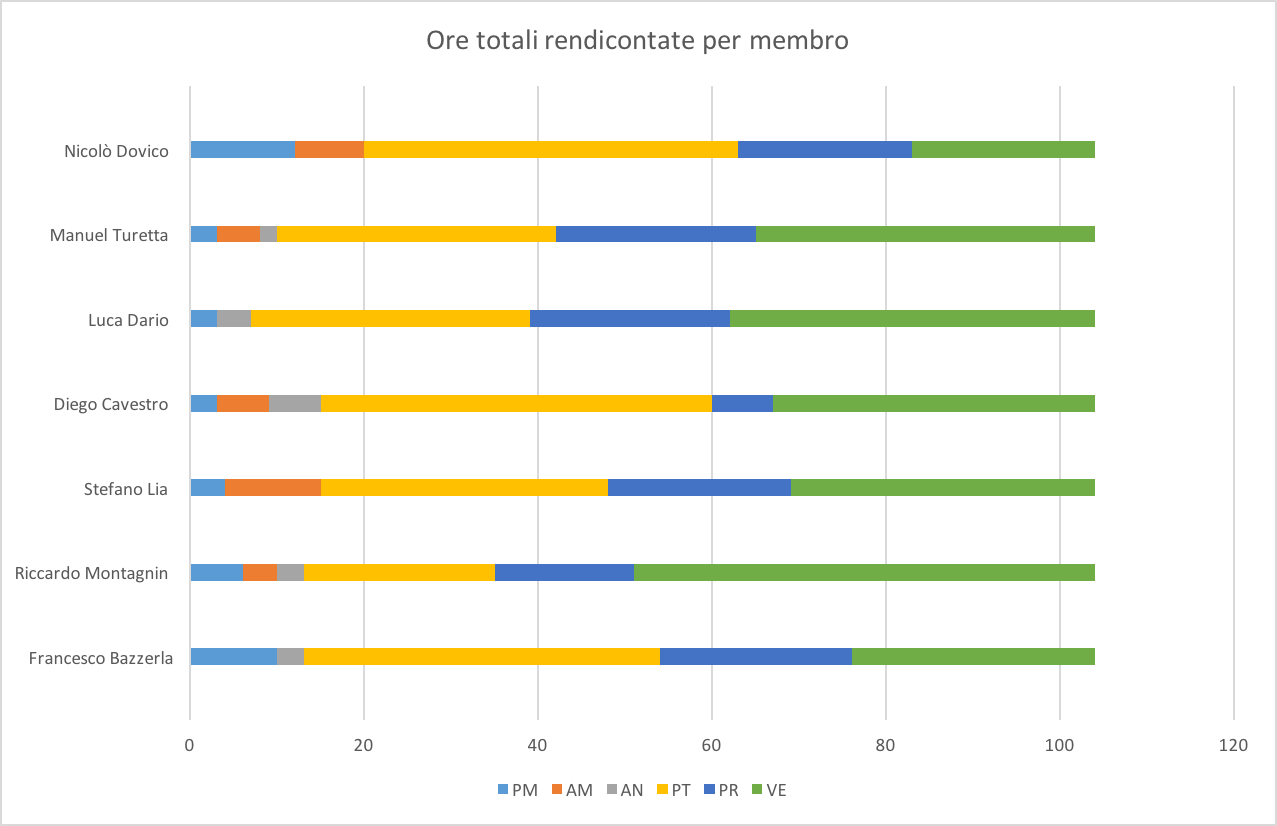
\includegraphics[scale=0.7]{Immagini/GraficiPianoLavoro/TOT.png}
	\caption{Incidenza ore totali per membro}
\end{figure}
\newpage
\section{Prospetto economico}
In questo paragrafo sono presentate, per ciascun periodo del progetto, le ore di impegno calcolate a preventivo per i ruoli coinvolti, divise tra ore di lavoro e ore contabilizzate.\\
 Si ricorda che il periodo di \ARM\ non è a carico del \termine{committente} e quindi non sarà considerata nel calcolo del preventivo.
 
\subsection{\ARD}
Nel periodo riguardante la fase di \ARD\ le ore tra i ruoli sono state divise nel seguente modo:

\begin{table}[h]
	\begin{center}
		\begin{tabular}{|l|c|c|}
			\hline
			\textbf{Ruolo}	& \textbf{Ore} & \textbf{Costo} \\
			\hline
			\textit{\Pm} &	5	&	 150	\\
			\hline
			\textit{\Am}	&	5	&	 100	\\
			\hline
			\textit{\An}	&	18	&	 450	\\
			\hline
			\textit{\Ver}	 & 11	&	 165	\\
			\hline
			\textbf{Totale} &	 39	&	865	\\
			\hline
		\end{tabular}
	\end{center}
	\caption{Incidenza ore su costo per ruolo, \ARD}
\end{table}

\begin{figure}[H]
	\centering 
	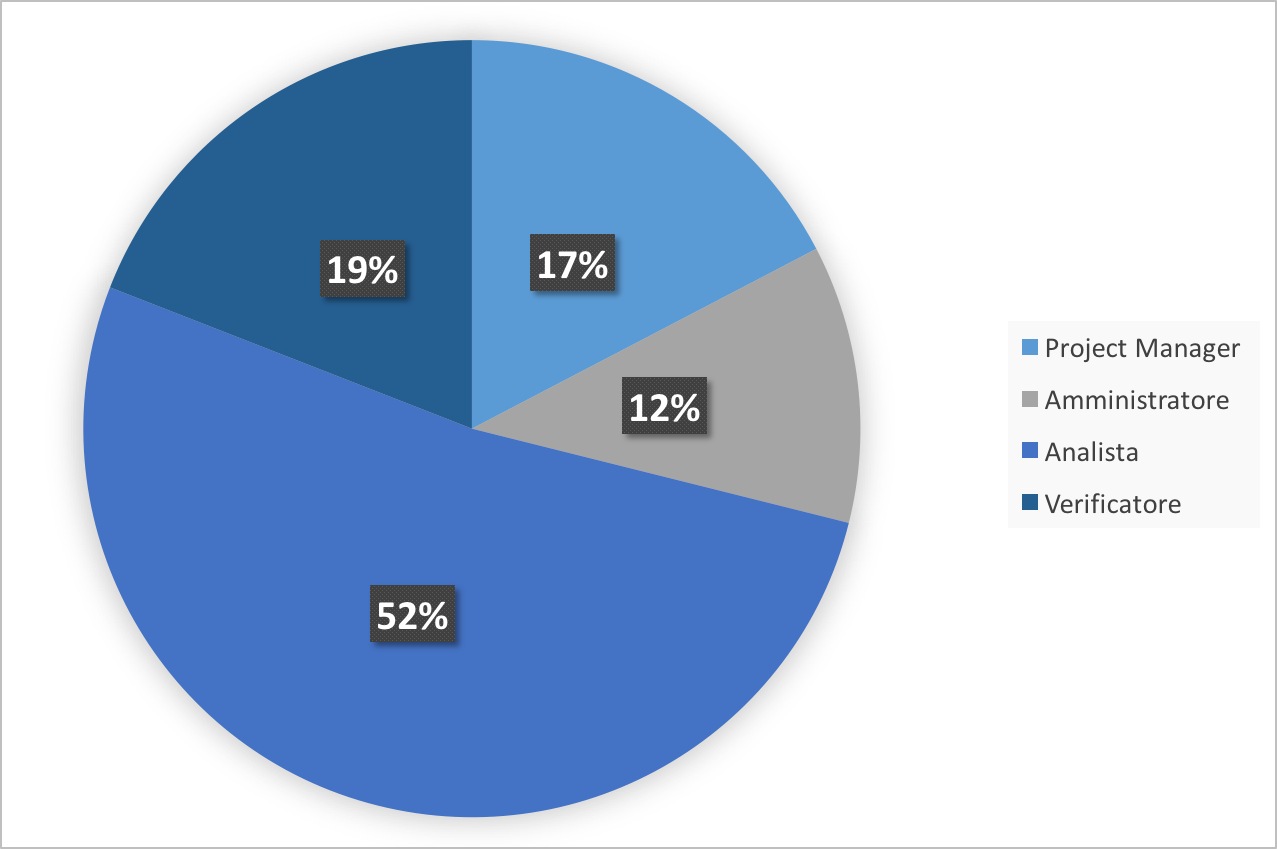
\includegraphics[scale=0.7]{Immagini/GraficiTorteSezione6/ARD.png}
	\caption{Costo per ruolo, \ARD}
\end{figure}

\newpage
\subsection{\PA}
Nel periodo riguardante la \PA\ le ore tra i ruoli sono state divise nel seguente modo:

\begin{table}[h]
	\begin{center}
		\begin{tabular}{|l|c|c|}
			\hline
			\textbf{Ruolo}	& \textbf{Ore} &	\textbf{Costo}	 \\
			\hline
			\textit{\Pm}	&	6	&	180		\\
			\hline
			\textit{\Am}	&	8	&	160		\\
			\hline
			\textit{\Prog}	&	129	&	2838	\\
			\hline
			\textit{\Ver}	&	62	&	930	\\
			\hline
			\textbf{Totale}	&	205	&	4108	\\
			\hline
		\end{tabular}
	\end{center}
	\caption{Incidenza ore su costo per ruolo, \PA}
\end{table}

\begin{figure}[H]
	\centering 
	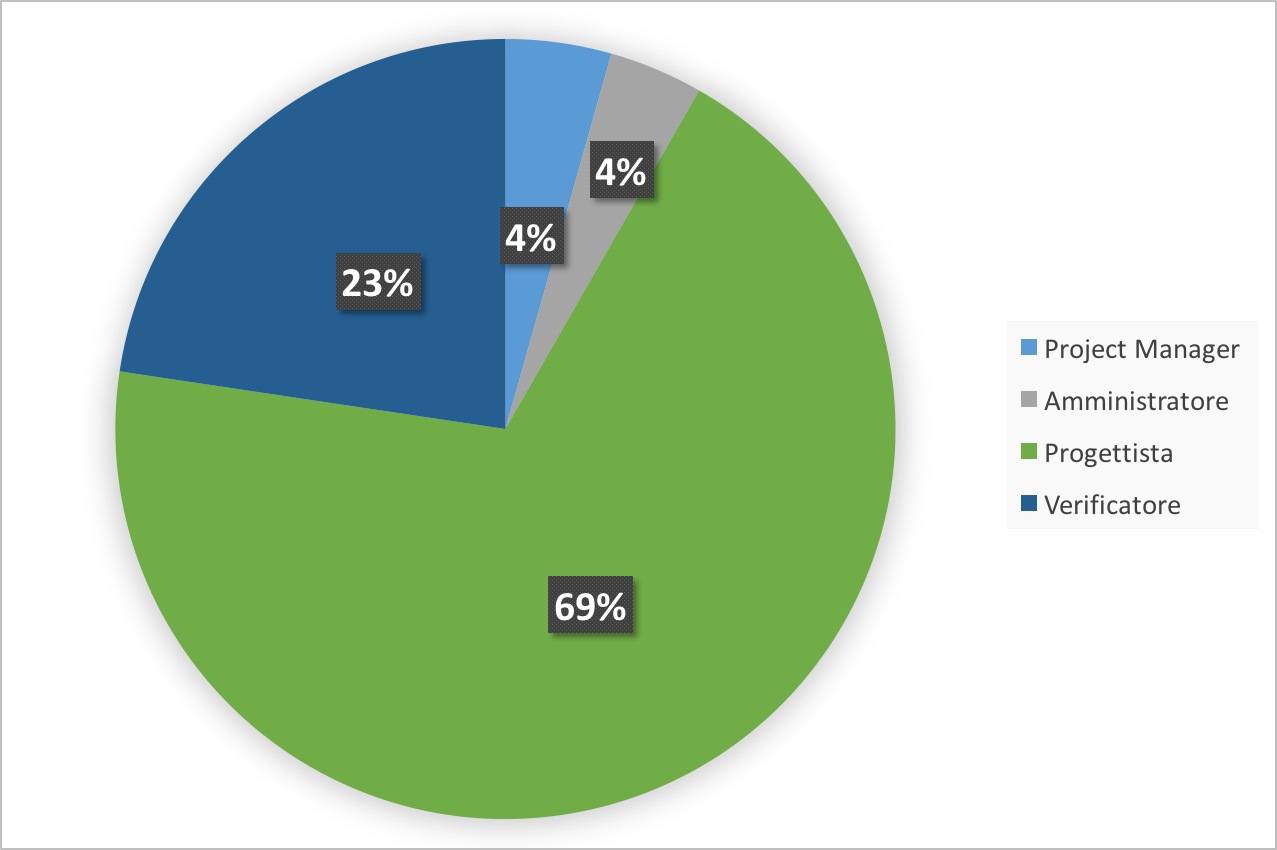
\includegraphics[scale=0.7]{Immagini/GraficiTorteSezione6/PA.png}
	\caption{Costo per ruolo, \PA}
\end{figure}

\newpage
\subsection{\PD}
Nel periodo riguardante la \PD\ le ore tra i ruoli sono state divise nel seguente modo:

\begin{table}[h]
	\begin{center}
		\begin{tabular}{|l|c|c|}
			\hline
			\textbf{Ruolo}	& \textbf{Ore} &	\textbf{Costo}	 \\
			\hline
			\textit{\Pm}	&	7	&	210		\\
			\hline
			\textit{\Am}	&	7	&	140		\\
			\hline
			\textit{\Prog}	&	76	&	1672	\\
			\hline
			\textit{\Ver}	&	38	&	570		\\
			\hline
			\textbf{Totale}	&	128	&	2592	\\
			\hline
		\end{tabular}
	\end{center}
	\caption{Incidenza ore su costo per ruolo, \PD}
\end{table}

\begin{figure}[H]
	\centering 
	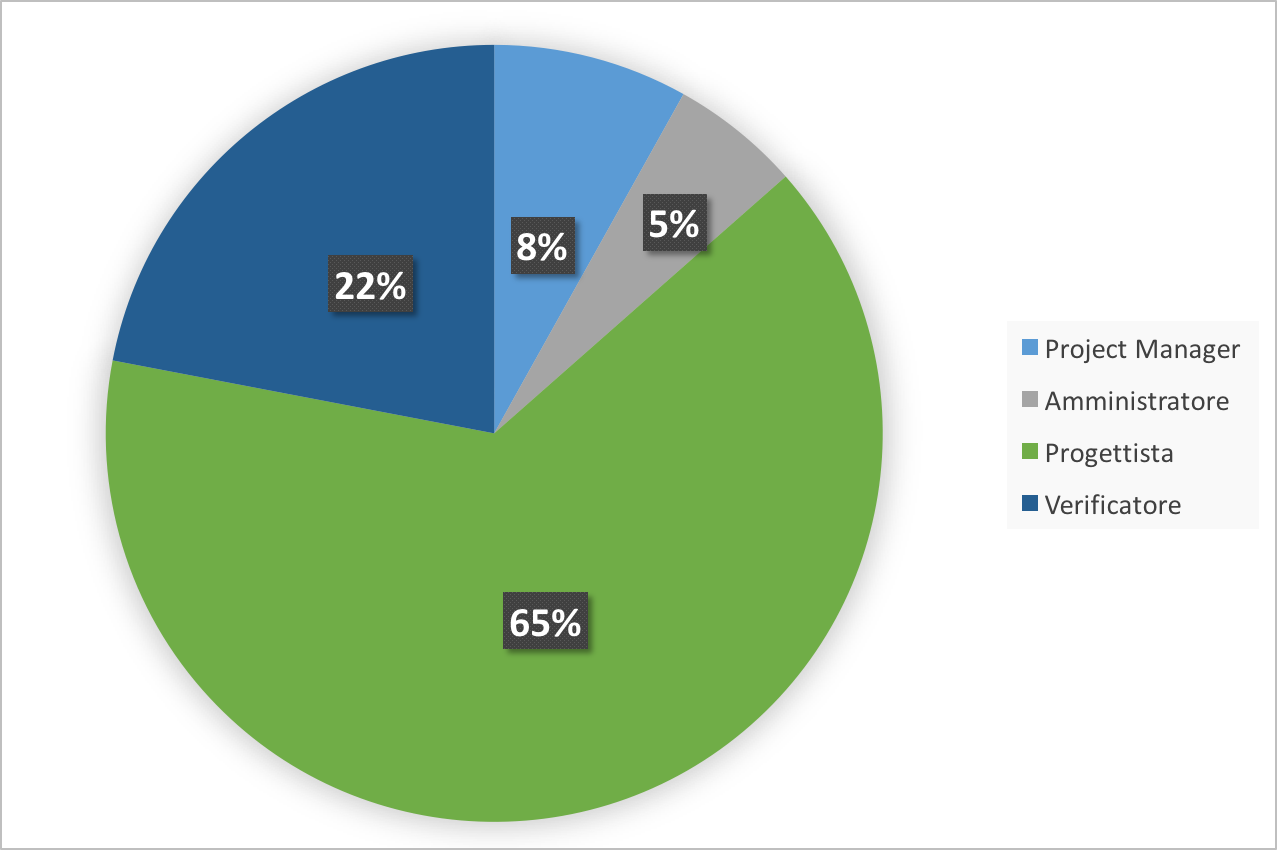
\includegraphics[scale=0.7]{Immagini/GraficiTorteSezione6/PD.png}
	\caption{Costo per ruolo, \PD}
\end{figure}

\newpage
\subsection{\COD}
Nel periodo riguardante la \COD\ le ore tra i ruoli sono state divise nel seguente modo:

\begin{table}[h]
	\begin{center}
		\begin{tabular}{|l|c|c|}
			\hline
			\textbf{Ruolo}	& \textbf{Ore} &	\textbf{Costo}	 \\
			\hline
			\textit{\Pm}	&	11	&	330		\\
			\hline
			\textit{\Am}	&	6	&	120		\\
			\hline
			\textit{\Prog}	&	21	&	462		\\
			\hline
			\textit{\Progr}	&	132	&	1980	\\
			\hline
			\textit{\Ver}	&	60	&	900	\\
			\hline
			\textbf{Totale}	&	230	&	3792	\\
			\hline
		\end{tabular}
	\end{center}
	\caption{Incidenza ore su costo per ruolo, \COD}
\end{table}

\begin{figure}[H]
	\centering 
	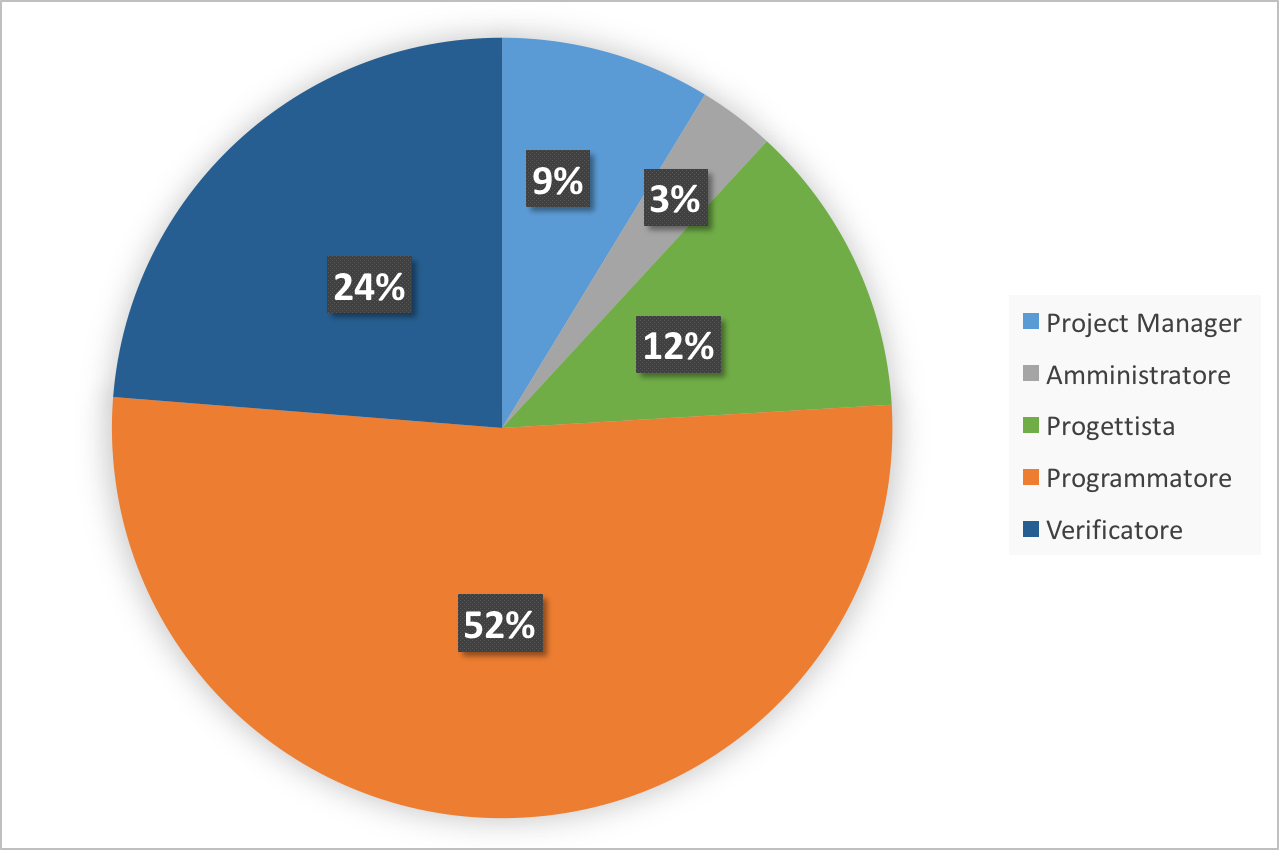
\includegraphics[scale=0.7]{Immagini/GraficiTorteSezione6/COD.png}
	\caption{Costo per ruolo, \COD}
\end{figure}

\newpage
\subsection{\VV}
Nel periodo riguardante la \VV\ le ore tra i ruoli sono state divise nel seguente modo:

\begin{table}[h]
	\begin{center}
		\begin{tabular}{|l|c|c|}
			\hline
			\textbf{Ruolo}	& \textbf{Ore} &	\textbf{Costo}	 \\
			\hline
			\textit{\Pm}	&	12	&	360		\\
			\hline
			\textit{\Am}	&	8	&	160		\\
			\hline
			\textit{\Prog}	&	22	&	484	\\
			\hline
			\textit{\Ver}	&	84	&	1260	\\
			\hline
			\textbf{Totale}	&	126	&	2264	\\
			\hline
		\end{tabular}
	\end{center}
	\caption{Incidenza ore su costo per ruolo, \VV}
\end{table}

\begin{figure}[H]
	\centering 
	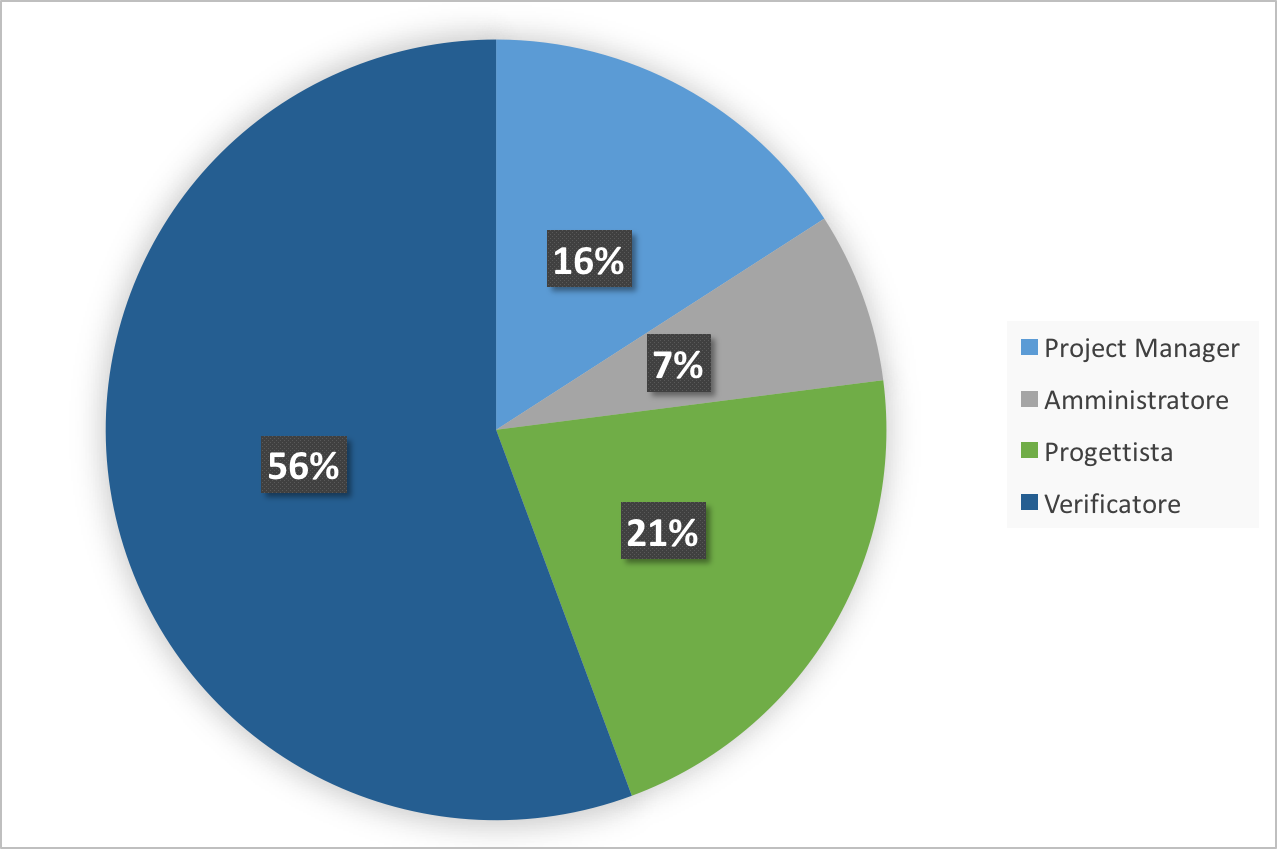
\includegraphics[scale=0.7]{Immagini/GraficiTorteSezione6/VV.png}
	\caption{Costo per ruolo, \VV}
\end{figure}

\newpage
\subsection{Totale}
\subsubsection{Ore totali}
Le ore totali, previste per la realizzazione dell'intero progetto, comprese le ore di investimento, sono riportate nella tabella seguente.

\begin{table}[h]
	\begin{center}
		\begin{tabular}{|l|c|c|c|}
			\hline
			\textbf{Ruolo}	& \textbf{Ore} &	\textbf{Ore remunerabili}	 &\textbf{Costo} \\
			\hline
			\textit{\Pm}	&	67	&	41	&	1230	\\
			\hline
			\textit{\Am}	&	54	&	34	&	680	\\
			\hline
			\textit{\An}	&	91	&	18	&	450	\\
			\hline
			\textit{\Prog}	&	248	&	248	&	5456	\\
			\hline
			\textit{\Progr}	&	132	&	132	&	1980	\\
			\hline
			\textit{\Ver}	&	311	&	255	&	3825	\\
			\hline
			\textbf{Totale}	&	903	&	728	&	13621	\\
			\hline
		\end{tabular}
	\end{center}
	\caption{Costo totale per ruolo}
\end{table}

\begin{figure}[H]
	\centering 
	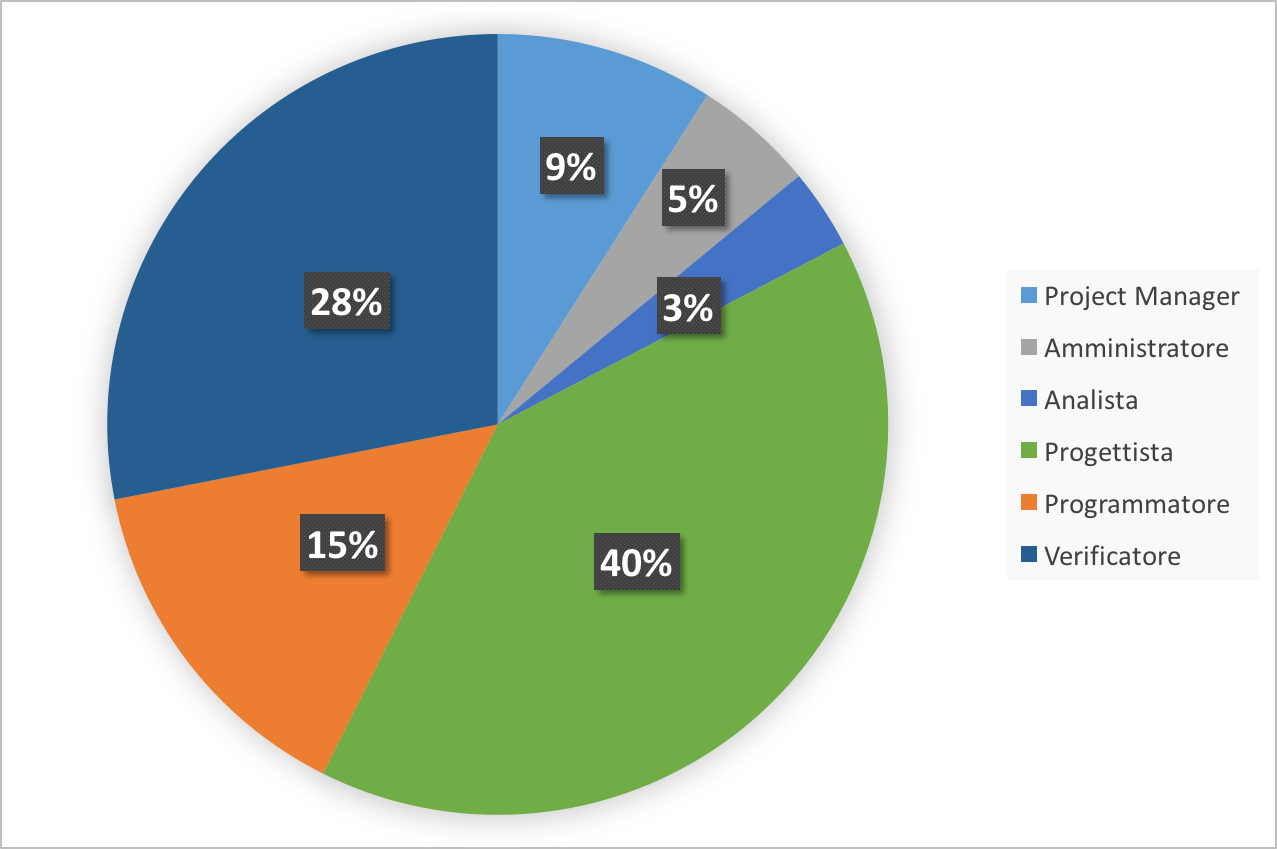
\includegraphics[scale=0.7]{Immagini/GraficiTorteSezione6/TOT.png}
	\caption{Costo totale per ruolo}
\end{figure}

\subsubsection{Conclusioni}
Il costo totale del progetto, indicato nella tabella 20, viene arrotondato a \textbf{\euro 13621}.\\
\newpage
\begin{appendices}


\section{Organigramma}
\subsection{Redazione}
\begin{table}[htbp]
	\begin{center}
		\setlength{\extrarowheight}{\jot}
		\begin{tabular}{|>{\centering}m{3cm}|>{\centering}m{2cm}|>{\centering\arraybackslash}m{3cm}|}
			\hline
			\textbf{Nominativo} & \textbf{Data di redazione} & \textbf{Firma} \\[1ex]
			\hline
			 \SL & 17/12/2017 & \SLFirma \\[1ex]
			\hline
			
			 \FB & 17/12/2017 & \FBFirma \\[1ex]
			\hline
		\end{tabular}
	\end{center}
	\caption{Redazione}
\end{table}

\subsection{Approvazione}
\begin{table}[htbp]
	\begin{center}
		\setlength{\extrarowheight}{\jot}
		\begin{tabular}{|>{\centering}m{3cm}|>{\centering}m{2cm}|>{\centering\arraybackslash}m{3cm}|}
			\hline
			\textbf{Nominativo} & \textbf{Data di redazione} & \textbf{Firma} \\[1ex]
			\hline
			 \LD & 08/01/2016 & \LDFirma \\[1ex]
			\hline
		\end{tabular}
	\end{center}
	\caption{Approvazione}
\end{table}

\newpage
\subsection{Accettazione dei componenti}
\begin{table}[!htbp]
	\begin{center}
		\setlength{\extrarowheight}{\jot}
		\begin{tabular}{|>{\centering}m{3cm}|>{\centering}m{2cm}|>{\centering\arraybackslash}m{3cm}|}
			\hline
			\textbf{Nominativo} & \textbf{Data di redazione} & \textbf{Firma} \\[1ex]
			\hline
			 \RM & 08/01/2017 & \RMFirma \\[1ex]
			\hline
			 \FB & 08/01/2017 & \FBFirma \\[1ex]
			\hline
			 \DC & 08/01/2017 & \DCFirma \\[1ex]
			\hline
			 \SL & 08/01/2017 & \SLFirma \\[1ex]
			\hline
			 \LD & 08/01/2017 & \LDFirma \\[1ex]
			\hline
			 \MT & 08/01/2017 & \MTFirma \\[1ex]
			 \hline
			 \ND & 08/01/2017 & \NDFirma \\[1ex]
			\hline
		\end{tabular}
	\end{center}
	\caption{Accettazione dei componenti}
\end{table}

\subsection{Componenti}
\begin{table}[!htbp]
	\begin{center}
		\setlength{\extrarowheight}{\jot}
		\begin{tabular}{|>{\centering}m{4cm}|>{\centering}m{2cm}|>{\centering}m{6.5cm} | >{\centering\arraybackslash}m{3cm}|}
			\hline
			\textbf{Nominativo} & \textbf{Matricola} & \textbf{Indirizzo di posta elettronica} & \textbf{Ruoli} \\[1ex]
			\hline
	 		\RM	& 1100577 & \href{mailto:riccardo.montagnin@studenti.unipd.it}{riccardo.montagnin@studenti.unipd.it} 	& \Pm, \An, \Ver \\[1ex]
			\hline
			\FB		& 1097417	& \href{mailto:francesco.bazzerla@studenti.unipd.it}{francesco.bazzerla@studenti.unipd.it} 			& \Am{}, \An{}, \Ver\	\\[1ex]
			\hline
			\DC		& 1094301	& \href{mailto:diego.cavestro.1@studenti.unipd.it}{diego.cavestro.1@studenti.unipd.it} 	& \Am{}, \An{}, \Ver\ 	\\[1ex]
			\hline
			\SL 		& 1097641	& \href{mailto:stefano.lia@studenti.unipd.it}{stefano.lia@studenti.unipd.it} 	& \Pm{}, \Am{}, \An\	\\[1ex]
			\hline
			\LD		& 1097935	& \href{mailto:luca.dario.1@studenti.unipd.it}{luca.dario.1@studenti.unipd.it} 			& \Pm{}, \Am{}, \An\ 	\\[1ex]
			\hline
			\MT		& 1103106	& \href{mailto:manuel.turetta.2@studenti.unipd.it}{manuel.turetta.2@studenti.unipd.it} 	& \Ver{}, \An\ 	\\[1ex]
			\hline
			\ND		& 1102846	& \href{mailto:nicolo.dovico@studenti.unipd.it}{nicolo.dovico@studenti.unipd.it} &  \Am{}, \An\ \\[1ex]
			\hline	
		\end{tabular}
	\end{center}
	\caption{Componenti}
\end{table}

\end{appendices}

\end{document}